% Created 2023-08-03 Thu 22:15
\documentclass[9pt, b5paper]{article}
\usepackage{xeCJK}
\usepackage[T1]{fontenc}
\usepackage{bera}
\usepackage[scaled]{beraserif}
\usepackage[scaled]{berasans}
\usepackage[scaled]{beramono}
\usepackage[cache=false]{minted}
\usepackage{xltxtra}
\usepackage{graphicx}
\usepackage{xcolor}
\usepackage{multirow}
\usepackage{multicol}
\usepackage{float}
\usepackage{textcomp}
\usepackage{algorithm}
\usepackage{algorithmic}
\usepackage{latexsym}
\usepackage{natbib}
\usepackage{geometry}
\geometry{left=1.2cm,right=1.2cm,top=1.5cm,bottom=1.2cm}
\usepackage[xetex,colorlinks=true,CJKbookmarks=true,linkcolor=blue,urlcolor=blue,menucolor=blue]{hyperref}
\newminted{common-lisp}{fontsize=\footnotesize} 
\author{deepwaterooo}
\date{\today}
\title{ET 框架学习笔记(五)--网络交互相关与Actor 机制}
\hypersetup{
  pdfkeywords={},
  pdfsubject={},
  pdfcreator={Emacs 28.2 (Org mode 8.2.7c)}}
\begin{document}

\maketitle
\tableofcontents


\section{StartConfigComponent: 找【各种服】的起始初始化地址}
\label{sec-1}
\begin{itemize}
\item 现在,先特殊重点理解:一台【服务端】物理机起来,N 核 N 进程里【主线程 Process 场景】的启动过程。
\item 【服务端、各服务器的配置、启动初始化】:是这个模块想要总结的内容。这个模块,因为框架重构里所接入的【路由器系统】的整合(感觉起来,就是通过网络,一台台服务端的服务器起来,一台台起来的服务器都向某个路由服,如同各客户端实时向位置服更新客户端的位置信息般,各小服专职服都向路由服上班打卡?要把这些看明白),让活宝妹理解起这个模块来显得相对困难,大概明天上午一上午的时间,都会花在这个模块上。
\end{itemize}
\subsection{OptionAttribute: 系统里的标签属性。}
\label{sec-1-1}
\begin{itemize}
\item 那么就是,命令行相关的。也就是ET 框架里所封装的,可以命令行,发布命令,启动【服务端】时的配置相关。【快看懂了吧。爱表哥,爱生活!!!任何时候,亲爱的表哥的活宝妹就是一定要、一定会嫁给活宝妹的亲爱的表哥!!!爱表哥,爱生活!!!】
\begin{minted}[fontsize=\scriptsize,linenos=false]{csharp}
namespace CommandLine {
    // 【CommandLine】:那么就是,命令行相关的。也就是ET 框架里所封装的,可以命令行,发布命令,启动【服务端】时的配置相关
    [AttributeUsage(AttributeTargets.Property, AllowMultiple = false, Inherited = true)]
    public sealed class OptionAttribute : BaseAttribute {
        public OptionAttribute();
        public OptionAttribute(string longName);
        public OptionAttribute(char shortName);
        public OptionAttribute(char shortName, string longName);
        public string LongName { get; }
        public string ShortName { get; }
        public string SetName { get; set; }
        public char Separator { get; set; }
        public string Group { get; set; }
    }
}
\end{minted}
\end{itemize}
\subsection{Options 单例类:}
\label{sec-1-2}
\begin{itemize}
\item 不知道这个单例类,是什么时候生成,什么情况下值会发生变化?跟命令行相关的话,当命令行启动【服务端】时,会启动这个【单例类】吗?网上搜下。
\begin{minted}[fontsize=\scriptsize,linenos=false]{csharp}
public class Options: Singleton<Options> { // 这个【单例类】,确实还没能看懂。单例类,不是组件添加形式。把【OptionAttribute】标签看懂
    [Option("AppType", Required = false, Default = AppType.Server, HelpText = "AppType enum")]
    public AppType AppType { get; set; }
    [Option("StartConfig", Required = false, Default = "StartConfig/Localhost")]
    public string StartConfig { get; set; }
    [Option("Process", Required = false, Default = 1)]
    public int Process { get; set; }

    [Option("Develop", Required = false, Default = 0, HelpText = "develop mode, 0正式 1开发 2压测")]
    public int Develop { get; set; }
    [Option("LogLevel", Required = false, Default = 2)]
    public int LogLevel { get; set; }

    [Option("Console", Required = false, Default = 0)]
    public int Console { get; set; }
    // 进程启动是否创建该进程的scenes
    [Option("CreateScenes", Required = false, Default = 1)]
    public int CreateScenes { get; set; }
}
\end{minted}
\end{itemize}

\subsection{模块里所用到的几个。NET 里的接口, 以及自定义的框架底层辅助体系类等}
\label{sec-1-3}
\subsubsection{ISupportInitialize: 【初始化】的支持接口,就是提供了【初始化之前】【初始化之后】的回调,两个API}
\label{sec-1-3-1}
\begin{minted}[fontsize=\scriptsize,linenos=false]{csharp}
namespace System.ComponentModel {
    public interface ISupportInitialize {
        void BeginInit();
        void EndInit();
    }
}
\end{minted}
\subsubsection{IInvoke: 抽象类会在事件系统 EventSystem.cs 中被用到}
\label{sec-1-3-2}
\begin{minted}[fontsize=\scriptsize,linenos=false]{csharp}
public interface IInvoke {
    Type Type { get; }
}
public abstract class AInvokeHandler<A>: IInvoke where A: struct {
    public Type Type {
        get {
            return typeof (A);
        }
    }
    public abstract void Handle(A a);
}
public abstract class AInvokeHandler<A, T>: IInvoke where A: struct {
    public Type Type {
        get {
            return typeof (A);
        }
    }
    public abstract T Handle(A a);
}
\end{minted}
\subsubsection{ISingleton 单例类接口:框架最底层,有狠多必要的单例类包装,统一实现这个单例接口,就是抽象提纯到框架最底层封装}
\label{sec-1-3-3}
\begin{minted}[fontsize=\scriptsize,linenos=false]{csharp}
public interface ISingleton: IDisposable {
    void Register();
    void Destroy();
    bool IsDisposed();
}
public abstract class Singleton<T>: ISingleton where T: Singleton<T>, new() {
    private bool isDisposed;
    [StaticField]
    private static T instance;
    public static T Instance {
        get {
            return instance;
        }
    }
    void ISingleton.Register() {
        if (instance != null) 
            throw new Exception($"singleton register twice! {typeof (T).Name}");
        instance = (T)this;
    }
    void ISingleton.Destroy() {
        if (this.isDisposed) 
            return;
        this.isDisposed = true;
        instance.Dispose();
        instance = null;
    }
    bool ISingleton.IsDisposed() {
        return this.isDisposed;
    }
    public virtual void Dispose() {
    }
}
\end{minted}
\subsubsection{IMerge: 在Proto 相关的地方,某些类如StartProcessConfig.cs 会实现这个接口,进程中以消息的形式传递这部分原理也要弄懂}
\label{sec-1-3-4}
\begin{itemize}
\item 这个接口,框架里定义了,主要用来帮助实现【动态路由】的。动态路由:网络中的路由器彼此之间互相通信,传递各自的路由信息,利用收到的路由信息来『自动合并』更新和维护自己路由表的过程。【动态路由特点】:自动化程度高,减少管理任务,错误率较低,但是占用网络资源。
\item 它定义了一个合并接口。因为这模块类中的诸多 Protobuf 相关的标签,活宝妹想,它们应该是可以以消息的形式进程间传递的。
\item 那么如果服务端的配置可以以消息的形式进程间传递,它合并时,谁与谁,如何合并的?感觉狠复杂的样子,要解一解。。。它是用在【动态路由系统】的模块。当一个路由器自动每 10 分钟周期性去扫描周围是否存在路由器邻居的时候,会自动合并。用行话说是,动态路由是网络中路由器之间互相通信,传递路由信息,利用收到的路由信息更新路由表的过程。这里【更新路由表】,说的就是当扫到了周围存在的路由器邻居,就更新自己当前路由器的路由表Info 成员变量。
\item 它能实时的适应网络结构的变化。如果路由更新信息表明网络发生了变化,路由选择软件就会重新计算路由,并发出新的路由更新信息。这些信息通过各个网络,引起各路由器重新启动其路由算法,并更新各自的路由表以动态的反映网络拓扑的变化。
\item 因为关于进程间消息自动合并?的这一块儿不懂,可以去找一下,什么情况下会调用这个合并?
\end{itemize}
\begin{minted}[fontsize=\scriptsize,linenos=false]{csharp}
public interface IMerge {
    void Merge(object o);
}
\end{minted}
\subsection{ProtoObject: 继承自上面的系统接口,定义必要的回调抽象API}
\label{sec-1-4}
\begin{minted}[fontsize=\scriptsize,linenos=false]{csharp}
public abstract class ProtoObject: Object, ISupportInitialize {
    public object Clone() { // 【进程间可传递的消息】:为什么这里的复制过程,是先序列化,再反序列化?
        // 不明白:消息明明就是反序列化好的,为什么再来一遍:序列化、反序列化(虽然这个再一遍的过程是 ProtoBuf 里的序列化与反序列化方法)?
        // 翻到Protobuf 里的反序列化方法,去查看:ET 框架的封装里,
            // 在底层内存流上的反序列化方法时(ProtobufHelper.Deserialize()),会调用 ISupportInitialize 的EndInit()回调,序列化后可做的事的回调
            // 序列化前的回调,是哪里调用的?BeginInit() 回调在框架里,只有在MongoHelper.cs 的Json 序列化前,会调用;ProtoBuf 序列化前好像跳过了这个回调
            // 就是提供了两个接口:调用与不调用,还是分不同的序列化工具
        byte[] bytes = SerializeHelper.Serialize(this);
        return SerializeHelper.Deserialize(this.GetType(), bytes, 0, bytes.Length);
    }
    public virtual void BeginInit() {
    }
    public virtual void EndInit() {
    }
    public virtual void AfterEndInit() { // 这个回调,与上一个 EndInit() 区别是?
    }
}
\end{minted}
\subsection{ConfigLoader.cs: 【服务端】是理解接下来部分的基础。【客户端】有不同逻辑。所以要把两边的都看一下}
\label{sec-1-5}
\begin{itemize}
\item 这个类名奇怪的地方是:它明明是定义了两个Invoke 标签事件的触发回调逻辑,为什么它的名字叫的是ConfigLoader? 感觉是扫描程序域里所有的【Config】标签一样。。。
\item 【任何时候,亲爱的表哥的活宝妹就是一定要嫁给亲爱的表哥!!!爱表哥,爱生活!!!】
\item 这个文件的GetAllConfigBytes 类中的回调:会去事件系统拿程序域里所有标记【Config】标签的类型,并根据这些标签类型是否为四大单例类之一来确认读取配置的位置。就是四个单例管理类的配置位置会相对特殊一点儿。
\end{itemize}
\begin{minted}[fontsize=\scriptsize,linenos=false]{csharp}
[Invoke] // 激活系: 这个激活系是同属ET 强大的事件系统的一个标签和回调逻辑,处理两种类型: GetAllConfigBytes 和 GetOneConfigBytes
public class GetAllConfigBytes: AInvokeHandler<ConfigComponent.GetAllConfigBytes, Dictionary<Type, byte[]>> {
    public override Dictionary<Type, byte[]> Handle(ConfigComponent.GetAllConfigBytes args) {
        Dictionary<Type, byte[]> output = new Dictionary<Type, byte[]>();
        List<string> startConfigs = new List<string>() {
            "StartMachineConfigCategory",  // 涉及底层配置的几个单例类,为什么这四个单例类类型重要: Machine, Process 进程、Scene 场景, Zone 区
            "StartProcessConfigCategory", 
            "StartSceneConfigCategory", 
            "StartZoneConfigCategory",
        };
// 类型:这里,扫的是所有【Invoke】标签(好像不对),还是说如【Invoke(TimerInvokeType.ActorMessegaeSenderChecker)】之类的Invoke 标签的类型属性?去看一下方法定义
        HashSet<Type> configTypes = EventSystem.Instance.GetTypes(typeof (ConfigAttribute)); // 【Config】标签:返回程序域里所有的【Config】标签类型
        foreach (Type configType in configTypes) {
            string configFilePath;
            if (startConfigs.Contains(configType.Name)) { // 【单例管理类型】:有特异性的配置路径
                configFilePath = $"../Config/Excel/s/{Options.Instance.StartConfig}/{configType.Name}.bytes";    
            } else { // 其它:人海里的路人甲,读下配置就扔掉
                configFilePath = $"../Config/Excel/s/{configType.Name}.bytes";
            }
            output[configType] = File.ReadAllBytes(configFilePath);
        }
        return output;
    }
}
[Invoke]
public class GetOneConfigBytes: AInvokeHandler<ConfigComponent.GetOneConfigBytes, byte[]> {
    public override byte[] Handle(ConfigComponent.GetOneConfigBytes args) {
        // 【Invoke 回调逻辑】:从框架特定位置,读取特定属性条款的配置,返回字节数组
        byte[] configBytes = File.ReadAllBytes($"../Config/{args.ConfigName}.bytes");
        return configBytes;
    }
}
\end{minted}
\subsection{ConfigLoader:【客户端】}
\label{sec-1-6}
\begin{itemize}
\item 【客户端】与【服务端】不同的是,客户端需要区分当前的运行,是在编辑器模式下,还是真正运行在客户端设备(PC 平台)。编辑器模式下,如服务端,去特定的位置去读配置文件;而真正的客户端,就需要从热更新资源服务器(斗地主参考项目中,仍是有个其它语言的最小最精致热更新资源包专职服务器的,ET7 里好像没有了,而是放在一个特定的文件夹下?)服务端来下载配置资源包,读取资源包里的配置内容,并字典管理,
\end{itemize}
\begin{minted}[fontsize=\scriptsize,linenos=false]{csharp}
[Invoke]
public class GetAllConfigBytes: AInvokeHandler<ConfigComponent.GetAllConfigBytes, Dictionary<Type, byte[]>> {
    public override Dictionary<Type, byte[]> Handle(ConfigComponent.GetAllConfigBytes args) {
        Dictionary<Type, byte[]> output = new Dictionary<Type, byte[]>();
        HashSet<Type> configTypes = EventSystem.Instance.GetTypes(typeof (ConfigAttribute));
        if (Define.IsEditor) { // 【编辑器模式下】:
            string ct = "cs";
            GlobalConfig globalConfig = Resources.Load<GlobalConfig>("GlobalConfig"); // 加载全局模式:这里没有看懂
            CodeMode codeMode = globalConfig.CodeMode;
            switch (codeMode) {
                case CodeMode.Client:
                    ct = "c";
                    break;
                case CodeMode.Server:
                    ct = "s";
                    break;
                case CodeMode.ClientServer:
                    ct = "cs";
                    break;
                default:
                    throw new ArgumentOutOfRangeException();
            }
            List<string> startConfigs = new List<string>() {
                "StartMachineConfigCategory", 
                "StartProcessConfigCategory", 
                "StartSceneConfigCategory", 
                "StartZoneConfigCategory",
            };
            foreach (Type configType in configTypes) {
                string configFilePath;
                if (startConfigs.Contains(configType.Name)) {
                    configFilePath = $"../Config/Excel/{ct}/{Options.Instance.StartConfig}/{configType.Name}.bytes";    
                } else {
                    configFilePath = $"../Config/Excel/{ct}/{configType.Name}.bytes";
                }
                output[configType] = File.ReadAllBytes(configFilePath);
            }
        } else {
            using (Root.Instance.Scene.AddComponent<ResourcesComponent>()) { // <<<<<<<<<<<<<<<<<<<< 
                const string configBundleName = "config.unity3d";
                ResourcesComponent.Instance.LoadBundle(configBundleName);

                foreach (Type configType in configTypes) {
                    TextAsset v = ResourcesComponent.Instance.GetAsset(configBundleName, configType.Name) as TextAsset;
                    output[configType] = v.bytes;
                }
            }
        }
        return output;
    }
}
[Invoke]
public class GetOneConfigBytes: AInvokeHandler<ConfigComponent.GetOneConfigBytes, byte[]> {
    public override byte[] Handle(ConfigComponent.GetOneConfigBytes args) {
        // TextAsset v = ResourcesComponent.Instance.GetAsset("config.unity3d", configName) as TextAsset;
        // return v.bytes;
        throw new NotImplementedException("client cant use LoadOneConfig");
    }
}
\end{minted}
\subsection{ConfigComponent 组件:单例类。底层组件,负责服务端配置相关管理?}
\label{sec-1-7}
\begin{itemize}
\item 这个底层组件的内部,涉及ET 标签事件系统的扫描【Config】标签,并Invoke 相关(服务端的配置与启动?)这里花点儿时间,再进去把ET 事件系统中各小服服务端根据(excel? 等) 配置文件来加载和启动服务端(或是服务端的必要配置)的原理弄懂
\item 框架事件系统里,有对各种不同标签的处理逻辑。Invoke 同理。程序域加载时,它扫描和管理框架里的所有必要相关标签,同Invoke 标签同样有字典(套字典)纪录管理不同参数类型(args)的字典,字典里不同类型(type) 的激活处理器。对于特定的参数类型,type 类型,如果能够找到激活处理器,就会触发调用此激活回调,来作相应的处理。
\end{itemize}
\begin{minted}[fontsize=\scriptsize,linenos=false]{csharp}
public T Invoke<A, T>(int type, A args) where A: struct {
    // 先试着去拿,框架里这个【特定 args 类型】的所有标签申明过的 invokeHandlers
    if (!this.allInvokes.TryGetValue(typeof(A), out var invokeHandlers)) {
        throw new Exception($"Invoke error: {typeof(A).Name}");
    }
    // 再试着去拿,【特定类型 type】的 invokeHandler 处理器
    if (!invokeHandlers.TryGetValue(type, out var invokeHandler)) {
        throw new Exception($"Invoke error: {typeof(A).Name} {type}");
    }
    var aInvokeHandler = invokeHandler as AInvokeHandler<A, T>;
    if (aInvokeHandler == null) {
        throw new Exception($"Invoke error, not AInvokeHandler: {typeof(T).Name} {type}");
    }
    return aInvokeHandler.Handle(args); // 调用【Invoke】标签的相应处理回调逻辑
}
public void Invoke<A>(A args) where A: struct {
    Invoke(0, args);
}
public T Invoke<A, T>(A args) where A: struct {
    return Invoke<A, T>(0, args);
}
\end{minted}
\begin{itemize}
\item 框架最底层的封装原理如此。这里,更多的是需要去找当前配置系,激活处理器的具体实现逻辑(在ConfigLoader.cs 文件里,两个回调类类型),来理解这个初始化加载模块。
\item 感觉今天上午把目前看到的这些,读得还算比较透彻。【亲爱的表哥,活宝妹一定要嫁的亲爱的表哥!!!任何时候,亲爱的表哥的活宝妹就是一定要嫁给亲爱的表哥!!爱表哥,爱生活!!!】
\end{itemize}
\begin{minted}[fontsize=\scriptsize,linenos=false]{csharp}
// Config组件会扫描所有的有【Config】标签的配置,加载进来:它借助了两套加载系统,加载一个配置,与加载所有配置。而配置仍是通过【Config】标签来标记配置类型
public class ConfigComponent: Singleton<ConfigComponent> {
    public struct GetAllConfigBytes {  }
    public struct GetOneConfigBytes {
        public string ConfigName;// 只是用一个字符串来区分不同配置 
    }
    private readonly Dictionary<Type, ISingleton> allConfig = new Dictionary<Type, ISingleton>();
    public override void Dispose() {
        foreach (var kv in this.allConfig) {
            kv.Value.Destroy();
        }
    }
    public object LoadOneConfig(Type configType) {
        this.allConfig.TryGetValue(configType, out ISingleton oneConfig);// oneConfig:这里算是自定义变量的【申明与赋值】?
        if (oneConfig != null) {
            oneConfig.Destroy();
        } 
        // 跟进Invoke: 去看一下框架里事件系统,找到具体的激活回调逻辑定义类:ConfigLoader.cs, 去查看里面对 GetOneConfigBytes 类型的激活触发逻辑
        byte[] oneConfigBytes = EventSystem.Instance.Invoke<GetOneConfigBytes, byte[]>(new GetOneConfigBytes() {ConfigName = configType.FullName});
        object category = SerializeHelper.Deserialize(configType, oneConfigBytes, 0, oneConfigBytes.Length);
        ISingleton singleton = category as ISingleton;
        singleton.Register(); // 【单例类初始化】:如果已经初始化过,会抛异常;单例类只初始化一次
        this.allConfig[configType] = singleton; // 底层:管理类单例类,不同类型,各有一个。框架里就有上面看过的四大单例类
        return category;
    }
    public void Load() { // 【加载】:系统加载,程序域加载 
        this.allConfig.Clear(); // 清空
        // 【原理】:借助框架强大事件系统,扫描域里【Invoke|()】标签(2 种);根据参数类型,调用触发激活逻辑,到服务端特定路径特定文件中去读取所有相关配置,并返回字典
        Dictionary<Type, byte[]> configBytes = EventSystem.Instance.Invoke<GetAllConfigBytes, Dictionary<Type, byte[]>>(new GetAllConfigBytes());
        foreach (Type type in configBytes.Keys) {
            byte[] oneConfigBytes = configBytes[type];
            this.LoadOneInThread(type, oneConfigBytes);
        }
    }
    public async ETTask LoadAsync() { // 哪里会调用这个方法?Entry.cs 服务端起来的时候,会调用此底层组件,加载各单例管理类。细看一下这里服务端启动初始化逻辑
        this.allConfig.Clear();
        Dictionary<Type, byte[]> configBytes = EventSystem.Instance.Invoke<GetAllConfigBytes, Dictionary<Type, byte[]>>(new GetAllConfigBytes());
        using ListComponent<Task> listTasks = ListComponent<Task>.Create();
        foreach (Type type in configBytes.Keys) {
            byte[] oneConfigBytes = configBytes[type];
// 四大单例管理类(Machine,Process,Scene,Zone):每个单例类,开一个任务线路去完成?好像是这样的。
// 不明白为什么必须管理那四个,多不同场景可以位于同一进程,一台机器可以多核多进程?区区区。。。不明白
            Task task = Task.Run(() => LoadOneInThread(type, oneConfigBytes)); 
            listTasks.Add(task);
        }
        await Task.WhenAll(listTasks.ToArray());
    }

    private void LoadOneInThread(Type configType, byte[] oneConfigBytes) {
        object category = SerializeHelper.Deserialize(configType, oneConfigBytes, 0, oneConfigBytes.Length);
        lock (this) {
            ISingleton singleton = category as ISingleton;
            singleton.Register(); // 注册单例类:就是启动初始化一个单例类吧,框架里 Invoke 配置相关,有四大单例类
            this.allConfig[configType] = singleton;
        }
    }
}
\end{minted}
\subsection{ConfigSingleton<T>: ProtoObject, ISingleton}
\label{sec-1-8}
\begin{itemize}
\item 【配置单例泛型类】:实现ISingleton 接口,适用于各种不同类型的单例类管理(生成Register, 销毁Destroy, 以及加载完成后的回调管理)。
\end{itemize}
\begin{minted}[fontsize=\scriptsize,linenos=false]{java}
public abstract class ConfigSingleton<T>: ProtoObject, ISingleton where T: ConfigSingleton<T>, new() {
        [StaticField]
        private static T instance;
        public static T Instance {
            get {
                return instance ??= ConfigComponent.Instance.LoadOneConfig(typeof (T)) as T;
            }
        }
        void ISingleton.Register() {
            if (instance != null) {
                throw new Exception($"singleton register twice! {typeof (T).Name}");
            }
            instance = (T)this;
        }
        void ISingleton.Destroy() {
            T t = instance;
            instance = null;
            t.Dispose();
        }
        bool ISingleton.IsDisposed() {
            throw new NotImplementedException();
        }
        public override void AfterEndInit() { } // <<<<<<<<<<<<<<<<<<<< 一个回调接口API
        public virtual void Dispose() { }
    }
\end{minted}
\subsection{StartMachineConfig: 抓四大单例管理类中的一个来读一下}
\label{sec-1-9}
\begin{itemize}
\item 同样的命名空间,同一个文件,完全相同的类型,没弄明白的是,它为什么会在框架里出现两遍?是叫 partial-class, 可是这样的原理、两个文件的区别,以及用途,是在哪里是什么?
\item 这个单例类型只存在于【服务端】。但是ET 框架里,双端框架有多种不同运行模式。客户端可以作为独立客户端来运行,也可以作为双端模式运行(就是内自带一个服务端)。这里的服务端就同理,可是作为独立服务端,只作服务端,也可以作为客户端在双端运行模式中,客户端自身所携带的服务端来运行。所以,框架里它出现了两次。
\item 另一个问题是:这个类是 Generated (/Users/hhj/pubFrameWorks/ET/Unity/Assets/Scripts/Codes/Model/Generate/ClientServer/Config/StartMachineConfig.cs), 是框架自动生成的类,没有看懂。为什么框架会生成这个类?
\item 今天大概就只能读到这里了,剩下的明天上午再读。。。
\item 独立的服务端,框架生成的文件?作为客户端双端运行模式下的服务端:框架生成的文件?
\item Proto 相关的标签,各种各样的标签,看得懂的标签还好,不懂的Proto 标签看得。。。
\end{itemize}
\begin{minted}[fontsize=\scriptsize,linenos=false]{csharp}
[ProtoContract]
[Config]
public partial class StartMachineConfigCategory : ConfigSingleton<StartMachineConfigCategory>, IMerge { // 实现了这个合并接口
    [ProtoIgnore]
    [BsonIgnore]
    private Dictionary<int, StartMachineConfig> dict = new Dictionary<int, StartMachineConfig>();
    [BsonElement]
    [ProtoMember(1)]
    private List<StartMachineConfig> list = new List<StartMachineConfig>();
    public void Merge(object o) { // 实现接口里申明的方法
        StartMachineConfigCategory s = o as StartMachineConfigCategory;
        this.list.AddRange(s.list); // 这里就可以是,进程间可传递的消息,的自动合并
    }
    [ProtoAfterDeserialization]        
    public void ProtoEndInit() {
        foreach (StartMachineConfig config in list) {
            config.AfterEndInit();
            this.dict.Add(config.Id, config);
        }
        this.list.Clear();
        this.AfterEndInit();
    }
    public StartMachineConfig Get(int id) {
        this.dict.TryGetValue(id, out StartMachineConfig item);
        if (item == null) 
            throw new Exception($"配置找不到,配置表名: {nameof (StartMachineConfig)},配置id: {id}");
        return item;
    }
    public bool Contain(int id) {
        return this.dict.ContainsKey(id);
    }
    public Dictionary<int, StartMachineConfig> GetAll() {
        return this.dict;
    }
    public StartMachineConfig GetOne() {
        if (this.dict == null || this.dict.Count <= 0) 
            return null;
        return this.dict.Values.GetEnumerator().Current;
    }
}
[ProtoContract]
public partial class StartMachineConfig: ProtoObject, IConfig {
    [ProtoMember(1)]
    public int Id { get; set; }
    [ProtoMember(2)]
    public string InnerIP { get; set; }
    [ProtoMember(3)]
    public string OuterIP { get; set; }
    [ProtoMember(4)]
    public string WatcherPort { get; set; }
}
\end{minted}
\begin{itemize}
\item 也没有看出这两个文件有任何的区别,只是任何一个具备服务端功能的项目(.csproj)都还是需要这个文件而已。
\item 下面的文件就不放了,因为四大单例类(Machine, Process, Scene, Zone)还各不同,只抓一个只代表四分之一。。。得一个一个去分析。
\end{itemize}
\subsection{StartProcessConfig: 【任何时候,亲爱的表哥的活宝妹就是一定要嫁给亲爱的表哥!!!爱表哥,爱生活!!!】}
\label{sec-1-10}
\begin{itemize}
\item 按现有的理解,Machine 是一个相对大的单位;一个Machine 可以多核多进程多Process; 一个核一个进程一个Process 可以多线程多任务管理,一个Process 里可以并存多个不同的 SceneType 【并存多个相同或不同功能的小服:登录服,网关服,房间服。。】;Zone 区,还不懂算是什么意思
\item 与上面的Machine 不同的是,Process 真正涉及了Partial 的概念。同上一样,存在于【服务端】。可是因为 config 部分类的存在,框架里有四个文件。这里要把 partial 的原因弄明白.
\item 就是两个文件,分别存在于 Config 文件夹,与ConfigPartial 文件夹,不明白是为什么
\item 这里,把一个版本的源码先贴这里,改天再看
\end{itemize}
\begin{minted}[fontsize=\scriptsize,linenos=false]{csharp}
[ProtoContract]
[Config]
public partial class StartProcessConfigCategory : ConfigSingleton<StartProcessConfigCategory>, IMerge {
    [ProtoIgnore]
    [BsonIgnore]
    private Dictionary<int, StartProcessConfig> dict = new Dictionary<int, StartProcessConfig>();
    [BsonElement]
    [ProtoMember(1)]
    private List<StartProcessConfig> list = new List<StartProcessConfig>();
    public void Merge(object o) {
        StartProcessConfigCategory s = o as StartProcessConfigCategory;
        this.list.AddRange(s.list);
    }
    [ProtoAfterDeserialization]        
    public void ProtoEndInit() {
        foreach (StartProcessConfig config in list) {
            config.AfterEndInit();
            this.dict.Add(config.Id, config);
        }
        this.list.Clear();
        this.AfterEndInit();
    }
    public StartProcessConfig Get(int id) {
        this.dict.TryGetValue(id, out StartProcessConfig item);
        if (item == null) {
            throw new Exception($"配置找不到,配置表名: {nameof (StartProcessConfig)},配置id: {id}");
        }
        return item;
    }
    public bool Contain(int id) {
        return this.dict.ContainsKey(id);
    }
    public Dictionary<int, StartProcessConfig> GetAll() {
        return this.dict;
    }
    public StartProcessConfig GetOne() {
        if (this.dict == null || this.dict.Count <= 0) {
            return null;
        }
        return this.dict.Values.GetEnumerator().Current;
    }
}
[ProtoContract]
public partial class StartProcessConfig: ProtoObject, IConfig {
    [ProtoMember(1)]
    public int Id { get; set; }
    [ProtoMember(2)]
    public int MachineId { get; set; }
    [ProtoMember(3)]
    public int InnerPort { get; set; }
}
\end{minted}
\subsection{StartSceneConfig: ISupportInitialize 【各种服-配置,场景配置】}
\label{sec-1-11}
\begin{minted}[fontsize=\scriptsize,linenos=false]{csharp}
public partial class StartSceneConfig: ISupportInitialize {
    public long InstanceId;
    public SceneType Type; // 场景类型

    public StartProcessConfig StartProcessConfig {
        get {
            return StartProcessConfigCategory.Instance.Get(this.Process);
        }
    }
    public StartZoneConfig StartZoneConfig {
        get {
            return StartZoneConfigCategory.Instance.Get(this.Zone);
        }
    }
    // 内网地址外网端口,通过防火墙映射端口过来
    private IPEndPoint innerIPOutPort;
    public IPEndPoint InnerIPOutPort {
        get {
            if (innerIPOutPort == null) {
                this.innerIPOutPort = NetworkHelper.ToIPEndPoint($"{this.StartProcessConfig.InnerIP}:{this.OuterPort}");
            }
            return this.innerIPOutPort;
        }
    }
    // 外网地址外网端口
    private IPEndPoint outerIPPort;
    public IPEndPoint OuterIPPort {
        get {
            if (this.outerIPPort == null) {
                this.outerIPPort = NetworkHelper.ToIPEndPoint($"{this.StartProcessConfig.OuterIP}:{this.OuterPort}");
            }
            return this.outerIPPort;
        }
    }
    public override void AfterEndInit() {
        this.Type = EnumHelper.FromString<SceneType>(this.SceneType);
        InstanceIdStruct instanceIdStruct = new InstanceIdStruct(this.Process, (uint) this.Id);
        this.InstanceId = instanceIdStruct.ToLong();
    }
}
\end{minted}
\subsection{StartSceneConfigCategory : 【Matchs!】ConfigSingleton<StartSceneConfigCategory>, IMerge}
\label{sec-1-12}
\begin{itemize}
\item 为什么这个类,会是写了两遍呢?有什么不同?跟前面类似,存在于任何具备服务端功能的模块。【服务端】【双端】
\item 读里面的登录服,会知道它是如何管理登录服的(就是后面的例子,当它要拿登录服的地址的时候),它们是区服,就是分各个小区管理。如果集群是这个样子,大概匹配服也就是一样分小区管理了。
\item 那么这个配置管理里,因为我要用匹配服与地图服,也要对至少是匹配服进行管理。那么,我在申请匹配的时候,网关服才能拿到匹配服的地址。
\item 只在【服务端】存在。但是在双端模式、与服务端模式下,每种端有两个文件来定义这个类。。一个在【ProtoContract】里,可能可以进程间消息传递?一个在 ConfigPartial 文件夹里
\item 这里的部分类 partial-class 仍然是没弄明白。什么情况下使用哪个类,不同部分类的实现原理。
\item 【重构】:因为我现在还比较喜欢使用Unity 下自带的双端模式,可是暂时只改【双端模式 ClientServer】下的文件,另一个专职服务端可能晚点儿再补上去。不用昨天晚上一样每个文件都改。
\item 不知道下面的源码,属于端的两种模式、部分类的两个文件,四个中的哪一个?
\end{itemize}
\begin{minted}[fontsize=\scriptsize,linenos=false]{csharp}
// 配置文件处理,或是服务器启动相关类,以前都没仔细读过
public partial class StartSceneConfigCategory {
    public MultiMap<int, StartSceneConfig> Gates = new MultiMap<int, StartSceneConfig>();
    public MultiMap<int, StartSceneConfig> ProcessScenes = new MultiMap<int, StartSceneConfig>();
    public Dictionary<long, Dictionary<string, StartSceneConfig>> ClientScenesByName = new Dictionary<long, Dictionary<string, StartSceneConfig>>();
    public StartSceneConfig LocationConfig;
    public List<StartSceneConfig> Realms = new List<StartSceneConfig>();
    public List<StartSceneConfig> Matchs = new List<StartSceneConfig>(); // <<<<<<<<<<<<<<<<<<<< 添加管理
    public List<StartSceneConfig> Routers = new List<StartSceneConfig>();
    public List<StartSceneConfig> Robots = new List<StartSceneConfig>();
    public StartSceneConfig BenchmarkServer;

    public List<StartSceneConfig> GetByProcess(int process) {
        return this.ProcessScenes[process];
    }
    public StartSceneConfig GetBySceneName(int zone, string name) {
        return this.ClientScenesByName[zone][name];
    }
    public override void AfterEndInit() {
        foreach (StartSceneConfig startSceneConfig in this.GetAll().Values) {
            this.ProcessScenes.Add(startSceneConfig.Process, startSceneConfig);
                
            if (!this.ClientScenesByName.ContainsKey(startSceneConfig.Zone)) {
                this.ClientScenesByName.Add(startSceneConfig.Zone, new Dictionary<string, StartSceneConfig>());
            }
            this.ClientScenesByName[startSceneConfig.Zone].Add(startSceneConfig.Name, startSceneConfig);
                
            switch (startSceneConfig.Type) {
            case SceneType.Realm:
                this.Realms.Add(startSceneConfig);
                break;
            case SceneType.Gate:
                this.Gates.Add(startSceneConfig.Zone, startSceneConfig);
                break;
            case SceneType.Match:                  // <<<<<<<<<<<<<<<<<<<< 自己加的
                this.Matchs.Add(startSceneConfig); // <<<<<<<<<<<<<<<<<<<< 
                break;
            case SceneType.Location:
                this.LocationConfig = startSceneConfig;
                break;
            case SceneType.Robot:
                this.Robots.Add(startSceneConfig);
                break;
            case SceneType.Router:
                this.Routers.Add(startSceneConfig);
                break;
            case SceneType.BenchmarkServer:
                this.BenchmarkServer = startSceneConfig;
                break;
            }
        }
    }
}
\end{minted}

\section{Actor 消息相关:跟上个章节Net 相关一起总结,两个都不太清楚。放一起总结,希望都能够理解清楚}
\label{sec-2}
\begin{itemize}
\item 跨进程【发送消息】与【返回消息】的过程,总感觉无法完整地看通一遍。这个是狠久前的总结,还是修改更新下。等亲爱的表哥的活宝妹搬进新住处后,会改完所有的编译错误,会需要把这个重构游戏写完整。
\item ET中,正常的网络消息需要建立一个session链接来发送,这类消息对应的proto需要由IMessage,IResponse,IRequest来修饰。(这是最常规,感觉最容易理解的)
\item 另外还有一种消息机制,称为 \textbf{【Actor机制】} ,挂载了MailBoxComponent的实体会成为一个actor. 而向Actor发送消息可以根据实体的instanceId来发送,不需要自己建立session链接,这类消息在proto中会打上IActorRequest, IActorResponse, IActorMessage的注释,标识为Actor消息。这种机制极大简化了服务器间向Actor发送消息的逻辑,使得实体间通信更加灵活方便。
\item 上面的,自己去想明白,挂载了MailBoxComponent的组件实体,知道对方实体的 instanceId, 背后的封装原理,仍然是对方实体 instanceId 之类的生成得比较聪明,自带自家进程 id, 让MailBoxCompoent 能够方便拿到发向收消息的进程?忘记了,好像是这样的。就是本质上仍是第一种,但封装得狠受用户弱弱程序员方便实用。。。
\item 但有的时候实体需要在服务器间传递(这一块儿还没有涉入,可以简单理解为玩家 me 从加州地图,重入到了亲爱的表哥身边的地图,不嫁给亲爱的表哥就永远不再离开。 me 大概可以理解为从一个地图服搬家转移重入到了另一个地图服, me 所属的进程可能已经变了),每次传递都会实例化一个新的,其instanceId也会变,但实体的id始终不会变,所以为了应对实体传递的问题,增加了proto需要修饰为IActorLocationRequest, IActorLocationResponse, IActorLocationMessage的消息【这一块儿仍不懂,改天再捡】,它可以根据实体Id来发送消息,不受实体在服务器间传递的影响,很好的解决了上面的问题。
\end{itemize}
\subsection{ActorMessageSender: 知道对方的instanceId,使用这个类发actor消息}
\label{sec-2-1}
\begin{itemize}
\item Tcs 成员变量:精华在这里:因为内部自带一个IActorResponse 的异步任务成员变量,可以帮助实现异步消息的自动回复
\item 正是因为内部成员自带一个异步任务,所以会多一个成员变量,就是标记是否要抛异常。这是异步任务成员变量带来的
\begin{minted}[fontsize=\scriptsize,linenos=false]{csharp}
public readonly struct ActorMessageSender {
    public long ActorId { get; }
    public long CreateTime { get; } // 最近接收或者发送消息的时间
    public IActorRequest Request { get; }      // 结构体,也自动封装了,发送的消息
    public bool NeedException { get; }         // 这上下三行:就帮助实现,返回消息的自动回复的结构包装
    public ETTask<IActorResponse> Tcs { get; } // <<<<<<<<<<<<<<<<<<<< 精华在这里:因为内部自带一个IActorResponse 的异步任务成员变量,可以帮助实现异步消息的自动回复
    public ActorMessageSender(long actorId, IActorRequest iActorRequest, ETTask<IActorResponse> tcs, bool needException) { // tv ... 
        this.ActorId = actorId;
        this.Request = iActorRequest;
        this.CreateTime = TimeHelper.ServerNow();
        this.Tcs = tcs;
        this.NeedException = needException;
    }
}
\end{minted}
\end{itemize}
\subsection{ActorMessageSenderComponent: 这个组件里有个计时器自动计时的超时时段、特定超时类型的超时时长成员变量,背后有套计时器管理组件,自动检测消息的发送超时。}
\label{sec-2-2}
\begin{itemize}
\item 超时时间:这个组件有计时器自动计时和超时激活的逻辑,这里定义了这个组件类型的超时时长,在ActorMessageSenderComponentSystem.cs 文件的 \textbf{【Invoke(TimerInvokeType.ActorMessageSenderChecker)】} 标注的ActorMessageSenderChecker 里会用到,检测超时与否
\item \textbf{【组件里消息自动超时Timer 的计时器机制】} :
\begin{itemize}
\item long TimeoutCheckTimer 是个重复闹钟
\item \textbf{【TimerComponent】} :是框架里的单例类,那么应该是,框架里所有的 Timer 定时计时器,应该是由这个单例管理类统一管理。那么这个组件应该能够负责相关逻辑。
\begin{minted}[fontsize=\scriptsize,linenos=false]{csharp}
[ComponentOf(typeof(Scene))]
public class ActorMessageSenderComponent: Entity, IAwake, IDestroy {
// 超时时间:这个组件有计时器自动计时和超时激活的逻辑,这里定义了这个组件类型的超时时长,在【Invoke(TimerInvokeType.ActorMessageSenderChecker)】标注的ActorMessageSenderChecker 里会用到,检测超时与否
    public const long TIMEOUT_TIME = 40 * 1000;
    public static ActorMessageSenderComponent Instance { get; set; }
    public int RpcId;
    public readonly SortedDictionary<int, ActorMessageSender> requestCallback = new SortedDictionary<int, ActorMessageSender>();
// 这个 long: 是重复闹钟的闹钟实例ID, 用来区分任何其它闹钟的
    public long TimeoutCheckTimer; 
    public List<int> TimeoutActorMessageSenders = new List<int>(); // 这桢更新里:待发送给的(接收者rpcId)接收者链表
}
\end{minted}
\end{itemize}
\end{itemize}
\subsection{ActorMessageSenderComponentSystem: 这个类底层封装比较多,功能模块因为是服务器端不太敦悉,多看几遍}
\label{sec-2-3}
\begin{itemize}
\item 这个类,可以看见ET7 框架更为系统化、消息机制的更为往底层或说更进一步的封装,就是今天下午看见的,以前的 handle() 或是 run() 方法,或回调实例 Action<T> reply, 现在的封装里,这些什么创建回复实例之类的,全部封装到了管理器或是帮助类
\item 如果发向同一个进程,则直接处理,不需要通过网络层。内网组件处理内网消息:这个分支可以再跟一下源码,理解一下重构的事件机制流程
\item 这个生成系,前半部分的计时器消息超时检测,看懂了;后半部分,还没看懂连能。今天上午能连多少连多少
\item 后半部分:是消息发送组件的相对底层逻辑。上层逻辑连通内外网消息,消息处理器,和读到消息发布事件后的触发调用等几个类。要把它们的连通流通原理弄懂。
\begin{minted}[fontsize=\scriptsize,linenos=false]{csharp}
[FriendOf(typeof(ActorMessageSenderComponent))]
public static class ActorMessageSenderComponentSystem {
    // 它自带个计时器,就是说,当服务器繁忙处理不过来,它就极有可能会自动超时,若是超时了,就返回个超时消息回去发送者告知一下,必要时它可以重发。而不超时,就正常基本流程处理了.那么,它就是一个服务端超负载下的自动减压逻辑
    [Invoke(TimerInvokeType.ActorMessageSenderChecker)] // 另一个新标签,激活系: 它标记说,这个激活系类,是 XXX 类型;紧跟着,就定义这个 XXX 类型的激活系类
    public class ActorMessageSenderChecker: ATimer<ActorMessageSenderComponent> {
        protected override void Run(ActorMessageSenderComponent self) { // 申明方法的接口是:ATimer<T> 抽象实现类,它实现了 AInvokeHandler<TimerCallback>
            try {
                self.Check(); // 调用组件自己的方法
             } catch (Exception e) {
                Log.Error($"move timer error: {self.Id}\n{e}");
            }
        }
    }
    [ObjectSystem]
    public class ActorMessageSenderComponentAwakeSystem: AwakeSystem<ActorMessageSenderComponent> {
// 【组件重复闹钟的设置】:实现组件内,消息的自动计时,超时触发Invoke 标签,调用相关逻辑来检测超时消息
        protected override void Awake(ActorMessageSenderComponent self) {
            ActorMessageSenderComponent.Instance = self;
// 这个重复闹钟,是消息自动计时超时过滤器的上下文连接桥梁
// 它注册的回调 TimerInvokeType.ActorMessageSenderChecker, 会每个消息超时的时候,都会回来调用 checker 的 Run()==>Check() 方法
// 应该是重复闹钟每秒重复一次,就每秒检查一次,调用一次Check() 方法来检查超时?是过滤器会给服务器减压;但这里的自动检测会把压分在各消息发送组件服务器上
// 这个重复间隔 1 秒钟的时间间隔,它计 1 秒钟开始,重复的逻辑是重复闹钟处理
            self.TimeoutCheckTimer = TimerComponent.Instance.NewRepeatedTimer(1000, TimerInvokeType.ActorMessageSenderChecker, self);
        }
    }//...
// Run() 方法:通过同步异常到ETTask, 通过ETTask 封装的抛异常方式抛出两类异常并返回;和对正常非异常返回消息,同步结果到ETTask, ETTask() 用触发调用注册过的非空回调
// 传进来的参数:是一个IActorResponse 实例,是有最小预处理(初始化了最基本成员变量:异常类型)、【写了个半好】的结果(异常)。结果还没同步到异步任务,待写;返回消息,待发送
    private static void Run(ActorMessageSender self, IActorResponse response) { 
        // 对于每个超时了的消息:超时错误码都是:ErrorCore.ERR_ActorTimeout, 所以会从发送消息超时异常里抛出异常,不用发送错误码【消息】回去,是抛异常
        if (response.Error == ErrorCore.ERR_ActorTimeout) { // 写:发送消息超时异常。因为同步到异步任务 ETTask 里,所以异步任务模块 ETTask会自动抛出异常
            self.Tcs.SetException(new Exception($"Rpc error: request, 注意Actor消息超时,请注意查看是否死锁或者没有reply: actorId: {self.ActorId} {self.Request}, response: {response}"));
            return;
        }
// 这个Run() 方法,并不是只有 Check() 【发送消息超时异常】一个方法调用。什么情况下的调用,会走到下面的分支?文件尾,有正常消息同步结果到ETTask 的调用 
// ActorMessageSenderComponent 一个组件,一次只执行一个(返回)消息发送任务,成员变量永远只管当前任务,
// 也是因为Actor 机制是并行的,一个使者一次只能发一个消息 ...
// 【组件管理器的执行频率, Run() 方法的调用频率】:要是消息太多,发不完怎么办呢?去搜索下面调用 Run() 方法的正常结果消息的调用处理频率。。。
        if (self.NeedException && ErrorCore.IsRpcNeedThrowException(response.Error)) { // 若是有异常(判断条件:消息要抛异常否?是否真有异常?),就先抛异常
            self.Tcs.SetException(new Exception($"Rpc error: actorId: {self.ActorId} request: {self.Request}, response: {response}"));
            return;
        }
        self.Tcs.SetResult(response); // 【写结果】:将【写了个半好】的消息,写进同步到异步任务的结果里;把异步任务的状态设置为完成;并触发必要的非空回调到发送者
        // 上面【异步任务 ETTask.SetResult()】,会调用注册过的一个回调,所以ETTask 封装,设置结果这一步,会自动触发调用注册过的一个回调(如果没有设置回调,因为空,就不会调用)
        // ETTask.SetResult() 异步任务写结果了,非空回调是会调用。非空回调是什么,是把返回消息发回去吗?不是。因为有独立的发送逻辑。
        // 再去想 IMHandler: 它是消息处理器。问题就变成是,当返回消息写好了,写好了一个完整的可以发送、待发送的消息,谁来处理的?有某个更底层的封装会调用这个类的发送逻辑。去把这个更底层的封装找出来,就是框架封装里,调用这个生成类Send() 方法的地方。
        // 这个服,这个自带计时器减压装配装置自带的消息处理器逻辑会处理?不是这个。减压装置,有发送消息超时,只触发最小检测,并抛发送消息超时异常给发送者告知,不写任何结果消息 
    }
    private static void Check(this ActorMessageSenderComponent self) {
        long timeNow = TimeHelper.ServerNow();
        foreach ((int key, ActorMessageSender value) in self.requestCallback) {
            // 因为是顺序发送的,所以,检测到第一个不超时的就退出
            // 超时触发的激活逻辑:是有至少一个超时的消息,才会【激活触发检测】;而检测到第一个不超时的,就退出下面的循环。
            if (timeNow < value.CreateTime + ActorMessageSenderComponent.TIMEOUT_TIME) 
                break;
            self.TimeoutActorMessageSenders.Add(key);
        }
// 超时触发的激活逻辑:是有至少一个超时的消息,才会【激活触发检测】;而检测到第一个不超时的,就退出上面的循环。
// 检测到第一个不超时的,理论上说,一旦有一个超时消息就会触发超时检测,但实际使用上,可能存在当检测逻辑被触发走到这里,实际中存在两个或是再多一点儿的超时消息?
        foreach (int rpcId in self.TimeoutActorMessageSenders) { // 一一遍历【超时了的消息】 :
            ActorMessageSender actorMessageSender = self.requestCallback[rpcId];
            self.requestCallback.Remove(rpcId);
            try { // ActorHelper.CreateResponse() 框架系统性的封装:也是通过对消息的发送类型与对应的回复类型的管理,使用帮助类,自动根据类型统一创建回复消息的实例
                // 对于每个超时了的消息:超时错误码都是:ErrorCore.ERR_ActorTimeout. 也就是,是个异常消息的回复消息实例生成帮助类
                IActorResponse response = ActorHelper.CreateResponse(actorMessageSender.Request, ErrorCore.ERR_ActorTimeout);
                Run(actorMessageSender, response); // 猜测:方法逻辑是,把回复消息发送给对应的接收消息的 rpcId
            } catch (Exception e) {
                Log.Error(e.ToString());
            }
        }
        self.TimeoutActorMessageSenders.Clear();
    }

    public static void Send(this ActorMessageSenderComponent self, long actorId, IMessage message) { // 发消息:这个方法,发所有类型的消息,最基接口
        if (actorId == 0) 
            throw new Exception($"actor id is 0: {message}");
        ProcessActorId processActorId = new(actorId);
        // 这里做了优化,如果发向同一个进程,则直接处理,不需要通过网络层
        if (processActorId.Process == Options.Instance.Process) { // 没看懂:这里怎么就说,消息是发向同一进程的了?
            NetInnerComponent.Instance.HandleMessage(actorId, message); // 原理清楚:本进程消息,直接交由本进程内网组件处理
            return;
        }
        Session session = NetInnerComponent.Instance.Get(processActorId.Process); // 非本进程消息,去走网络层
        session.Send(processActorId.ActorId, message);
    }
    public static int GetRpcId(this ActorMessageSenderComponent self) {
        return ++self.RpcId;
    }
    // 这个方法:只对当前进程的发送要求IActorResponse 的消息,封装自家进程的 rpcId, 也就是标明本进程发的消息,来自其它进程的返回消息,到时发到本进程。是特殊使用
    public static async ETTask<IActorResponse> Call(
        this ActorMessageSenderComponent self,
        long actorId,
        IActorRequest request,
        bool needException = true
        ) {
        request.RpcId = self.GetRpcId(); // 封装本进程的 rpcId 
        if (actorId == 0) throw new Exception($"actor id is 0: {request}");
        return await self.Call(actorId, request.RpcId, request, needException);
    }
    // 【艰森诲涩难懂!!】是更底层的实现细节,它封装帮助实现ET7 里消息超时自动过滤抛异常、返回消息的底层封装自动回复、封装了异步任务和必要成员变量来实现这些辅助过滤器等功能 
    public static async ETTask<IActorResponse> Call( // 跨进程发请求消息(要求回复):返回跨进程异步调用结果。是 await 关键字调用,用在异步方法里
        this ActorMessageSenderComponent self,
        long actorId,
        int rpcId,
        IActorRequest iActorRequest,
        bool needException = true
        ) {
        if (actorId == 0) 
            throw new Exception($"actor id is 0: {iActorRequest}");
// 对象池里:取一个异步任务。用这个异步作务实例,去创建下面的消息发送器实例。这里的 IActorResponse T 应该只是一个索引。因为前面看见系统扫描标签系创建返回实例,套到这个索引
        var tcs = ETTask<IActorResponse>.Create(true);
        // 下面,封装好消息发送器,交由消息发送组件管理;交由其管理,就自带消息发送计时超时过滤机制,实现服务器超负荷时的自动分压减压处理。一旦超时自动报废。。。
        self.requestCallback.Add(rpcId, new ActorMessageSender(actorId, iActorRequest, tcs, needException)); 
        self.Send(actorId, iActorRequest); // 把请求消息发出去:所有消息,都调用这个 
        long beginTime = TimeHelper.ServerFrameTime();
// 自己想一下的话:异步消息发出去,某个服会处理,有返回消息的话,这个服处理后会返回一个返回消息。
// 那么下面一行,不是等待创建 Create() 异步任务(同步方法狠快),而是等待这个处理发送消息的服,处理并返回来返回消息(是说,那个服,把处理结果同步到异步任务)
// 不是等异步任务的创建完成(同步方法狠快),实际是等处理发送消息的服,处理完并写好返回消息,同步到异步任务。
// 那个ETTask 里的回调 callback,是怎么回调的?这里Tcs 没有设置任何回调。ETTask 里所谓回调,是执行异步状态机的下一步,没有实际应用层面的回调意义
// 或说把返回消息的内容填好,【应该还没发回到消息发送者???】返回消息填好了,ETTask 异步任务的结果同步到位了,底层会自动发回来
// 【异步任务结果是怎么回来的?】是前面看过的IMHandler 的底层封装(AMRpcHandler 的抽象逻辑里)发送回来的。ET7 IMHandler 不是重构实现了返回消息的自动发送回复给发送者吗?再去看一遍。
        IActorResponse response = await tcs;  // 等待消息处理服处理完,写好同步好结果到异步任务、异步任务执行完成,状态为 Succeed
        long endTime = TimeHelper.ServerFrameTime();
        long costTime = endTime - beginTime;
        if (costTime > 200) 
            Log.Warning($"actor rpc time > 200: {costTime} {iActorRequest}");
        return response; // 返回:异步网络调用的结果
    }
// 【组件管理器的执行频率, Run() 方法的调用频率】:要是消息太多,发不完怎么办呢?去搜索下面调用 Run() 方法的正常结果消息的调用处理频率。。。
// 【ActorHandleHelper 帮助类】:老是调用这里的方法,要去查那个文件。【本质:内网消息处理器的处理逻辑,一旦是返回消息,就会调用 ActorHandleHelper, 会调用这个方法来处理返回消息】        
// 下面方法:处理IActorResponse 消息,也就是,发回复消息给收消息的人XX, 那么谁发,怎么发,就是这个方法的定义
    // 当是处理【同一进程的消息】:拿到的消息发送器就是当前组件自己,那么只要把结果同步到当前组件的Tcs 异步任务结果里,异步任务结果就会自动触发调用注册过的回调。全部流程结束
    public static void HandleIActorResponse(this ActorMessageSenderComponent self, IActorResponse response) {
        ActorMessageSender actorMessageSender;
// 下面取、实例化 ActorMessageSender 来看,感觉收消息的 rpcId, 与消息发送者 ActorMessageSender 成一一对应关系。上面的Call() 方法里,创建实例化消息发送者就是这么创始垢 
        if (!self.requestCallback.TryGetValue(response.RpcId, out actorMessageSender)) // 这里取不到,是说,这个返回消息的发送已经被处理了?
            return;
        self.requestCallback.Remove(response.RpcId); // 这个有序字典,就成为实时更新:随时添加,随时删除
        Run(actorMessageSender, response); // <<<<<<<<<<<<<<<<<<<< 
    }
}
\end{minted}
\item 几个类弄懂: ActorHandleHelper, 以及再上面的,NetInnerComponentOnReadEvent 事件发布等,上层调用的几座桥连通了,才算把整个流程弄懂了。
\item 现在不懂的就变成为:更为底层的,Session 会话框,socket 层的机制。但是因为它们更为底层,亲爱的表哥的活宝妹,现在把有限的精力投入支理解这个框架,适配自己的游戏比较重要。其它不太重要,或是更为底层的,改天有必要的时候再捡再看。【爱表哥,爱生活!!!任何时候,活宝妹就是一定要嫁给亲爱的表哥!!!爱表哥,爱生活!!!】
\end{itemize}
\subsection{LocationProxyComponent: 【位置代理组件】:为什么称它为代理?}
\label{sec-2-4}
\begin{itemize}
\item 就是有个启动类管理 StartSceneConfigCategory 类,它会分门别类地管理一些什么网关、注册登录服,地址服之类的东西。然后从这个里面拿位置服务器地址?大概意思是这样。写得可能不对。今天剩下一点儿时间,再稍微看一下
\item 感觉先前、上面仍然是写得不伦不类。总之,位置相关组件就是管理框架里各种可收发消息的实例,他们所在的(场景?位置?服务器地址?)相关位置信息。【亲爱的表哥的活宝妹就是一定要嫁给亲爱的表哥!!活宝妹只是在等:亲爱的表哥同活宝妹的一纸结婚证。活宝妹若是还没能嫁给亲爱的表哥,活宝妹就永远守候在亲爱的表哥的身边!!爱表哥,爱生活!!!】
\begin{minted}[fontsize=\scriptsize,linenos=false]{csharp}
[ComponentOf(typeof(Scene))]
public class LocationProxyComponent: Entity, IAwake, IDestroy {
    [StaticField]
    public static LocationProxyComponent Instance;
}
\end{minted}
\end{itemize}
\subsection{LocationProxyComponentSystem:}
\label{sec-2-5}
\begin{itemize}
\item 为什么要加那堆什么也没曾看懂的源码在那里?
\end{itemize}
\begin{minted}[fontsize=\scriptsize,linenos=false]{csharp}
// [ObjectSystem] awake() etc
\end{minted}
\subsection{:一个添加位置信息的请求消息处理类,示例}
\label{sec-2-6}

\subsection{ActorLocationSender: 知道对方的Id,使用这个类发actor消息}
\label{sec-2-7}
\begin{minted}[fontsize=\scriptsize,linenos=false]{csharp}
[ChildOf(typeof(ActorLocationSenderComponent))]
public class ActorLocationSender: Entity, IAwake, IDestroy {
    public long ActorId;
    public long LastSendOrRecvTime; // 最近接收或者发送消息的时间
    public int Error;
}
\end{minted}
\subsection{ActorLocationSenderComponent: 位置发送组件}
\label{sec-2-8}
\begin{minted}[fontsize=\scriptsize,linenos=false]{csharp}
 [ComponentOf(typeof(Scene))]
 public class ActorLocationSenderComponent: Entity, IAwake, IDestroy {
     public const long TIMEOUT_TIME = 60 * 1000;
     public static ActorLocationSenderComponent Instance { get; set; }
     public long CheckTimer;
 }
\end{minted}
\subsection{ActorLocationSenderComponentSystem: 这个类,也要明天上午再看一下}
\label{sec-2-9}
\begin{minted}[fontsize=\scriptsize,linenos=false]{csharp}
[Invoke(TimerInvokeType.ActorLocationSenderChecker)]
public class ActorLocationSenderChecker: ATimer<ActorLocationSenderComponent> {
    protected override void Run(ActorLocationSenderComponent self) {
        try {
            self.Check();
        }
        catch (Exception e) {
            Log.Error($"move timer error: {self.Id}\n{e}");
        }
    }
}
// [ObjectSystem] // ...
[FriendOf(typeof(ActorLocationSenderComponent))]
[FriendOf(typeof(ActorLocationSender))]
public static class ActorLocationSenderComponentSystem {
    public static void Check(this ActorLocationSenderComponent self) {
        using (ListComponent<long> list = ListComponent<long>.Create()) {
            long timeNow = TimeHelper.ServerNow();
            foreach ((long key, Entity value) in self.Children) {
                ActorLocationSender actorLocationMessageSender = (ActorLocationSender) value;
                if (timeNow > actorLocationMessageSender.LastSendOrRecvTime + ActorLocationSenderComponent.TIMEOUT_TIME) 
                    list.Add(key);
            }
            foreach (long id in list) {
                self.Remove(id);
            }
        }
    }
    private static ActorLocationSender GetOrCreate(this ActorLocationSenderComponent self, long id) {
        if (id == 0) 
            throw new Exception($"actor id is 0");
        if (self.Children.TryGetValue(id, out Entity actorLocationSender)) {
            return (ActorLocationSender) actorLocationSender;
        }
        actorLocationSender = self.AddChildWithId<ActorLocationSender>(id);
        return (ActorLocationSender) actorLocationSender;
    }
    private static void Remove(this ActorLocationSenderComponent self, long id) {
        if (!self.Children.TryGetValue(id, out Entity actorMessageSender)) 
            return;
        actorMessageSender.Dispose();
    }
    public static void Send(this ActorLocationSenderComponent self, long entityId, IActorRequest message) {
        self.Call(entityId, message).Coroutine();
    }
    public static async ETTask<IActorResponse> Call(this ActorLocationSenderComponent self, long entityId, IActorRequest iActorRequest) {
        ActorLocationSender actorLocationSender = self.GetOrCreate(entityId);
        // 先序列化好
        int rpcId = ActorMessageSenderComponent.Instance.GetRpcId();
        iActorRequest.RpcId = rpcId;
        long actorLocationSenderInstanceId = actorLocationSender.InstanceId;
        using (await CoroutineLockComponent.Instance.Wait(CoroutineLockType.ActorLocationSender, entityId)) {
            if (actorLocationSender.InstanceId != actorLocationSenderInstanceId) 
                throw new RpcException(ErrorCore.ERR_ActorTimeout, $"{iActorRequest}");
            // 队列中没处理的消息返回跟上个消息一样的报错
            if (actorLocationSender.Error == ErrorCore.ERR_NotFoundActor) 
                return ActorHelper.CreateResponse(iActorRequest, actorLocationSender.Error);
            try {
                return await self.CallInner(actorLocationSender, rpcId, iActorRequest);
            }
            catch (RpcException) {
                self.Remove(actorLocationSender.Id);
                throw;
            }
            catch (Exception e) {
                self.Remove(actorLocationSender.Id);
                throw new Exception($"{iActorRequest}", e);
            }
        }
    }
    private static async ETTask<IActorResponse> CallInner(this ActorLocationSenderComponent self, ActorLocationSender actorLocationSender, int rpcId, IActorRequest iActorRequest) {
        int failTimes = 0;
        long instanceId = actorLocationSender.InstanceId;
        actorLocationSender.LastSendOrRecvTime = TimeHelper.ServerNow();
        while (true) {
            if (actorLocationSender.ActorId == 0) {
                actorLocationSender.ActorId = await LocationProxyComponent.Instance.Get(actorLocationSender.Id);
                if (actorLocationSender.InstanceId != instanceId) 
                    throw new RpcException(ErrorCore.ERR_ActorLocationSenderTimeout2, $"{iActorRequest}");
            }
            if (actorLocationSender.ActorId == 0) {
                actorLocationSender.Error = ErrorCore.ERR_NotFoundActor;
                return ActorHelper.CreateResponse(iActorRequest, ErrorCore.ERR_NotFoundActor);
            }
            IActorResponse response = await ActorMessageSenderComponent.Instance.Call(actorLocationSender.ActorId, rpcId, iActorRequest, false);
            if (actorLocationSender.InstanceId != instanceId) 
                throw new RpcException(ErrorCore.ERR_ActorLocationSenderTimeout3, $"{iActorRequest}");
            switch (response.Error) {
                case ErrorCore.ERR_NotFoundActor: {
                    // 如果没找到Actor,重试
                    ++failTimes;
                    if (failTimes > 20) {
                        Log.Debug($"actor send message fail, actorid: {actorLocationSender.Id}");
                        actorLocationSender.Error = ErrorCore.ERR_NotFoundActor;
                        // 这里不能删除actor,要让后面等待发送的消息也返回ERR_NotFoundActor,直到超时删除
                        return response;
                    }
                    // 等待0.5s再发送
                    await TimerComponent.Instance.WaitAsync(500);
                    if (actorLocationSender.InstanceId != instanceId)
                        throw new RpcException(ErrorCore.ERR_ActorLocationSenderTimeout4, $"{iActorRequest}");
                    actorLocationSender.ActorId = 0;
                    continue;
                }
                case ErrorCore.ERR_ActorTimeout: 
                    throw new RpcException(response.Error, $"{iActorRequest}");
            }
            if (ErrorCore.IsRpcNeedThrowException(response.Error)) {
                throw new RpcException(response.Error, $"Message: {response.Message} Request: {iActorRequest}");
            }
            return response;
        }
    }
}
\end{minted}
\subsection{ActorHelper: 帮助创建IActorResponse 回复消息。狠简单}
\label{sec-2-10}
\begin{minted}[fontsize=\scriptsize,linenos=false]{csharp}
public static class ActorHelper {
    public static IActorResponse CreateResponse(IActorRequest iActorRequest, int error) {
        Type responseType = OpcodeTypeComponent.Instance.GetResponseType(iActorRequest.GetType());
        IActorResponse response = (IActorResponse)Activator.CreateInstance(responseType);
        response.Error = error;
        response.RpcId = iActorRequest.RpcId;
        return response;
    }
}
\end{minted}
\subsection{Actor 消息处理器:基本原理}
\label{sec-2-11}
\begin{itemize}
\item 消息到达MailboxComponent,MailboxComponent是有类型的,不同的类型邮箱可以做不同的处理。目前有两种邮箱类型GateSession跟MessageDispatcher。
\begin{itemize}
\item GateSession邮箱在收到消息的时候会立即转发给客户端。Actor 消息是指来自于服务端的消息(一定是来自于服务端的消息?Actor 一定是进程间,来自于其它服务端的?)。网关服是小区下所有用户的接收消息的代理。所以,网关服一旦收到服务端的返回消息,作为小区下所有用户的代理,就直接转发相应用户。【亲爱的表哥,永远是活宝妹的代理!任何时候,亲爱的表哥的活宝妹就是一定要嫁给亲爱的表哥!!爱表哥,爱生活!!!】
\item MessageDispatcher类型会再次对Actor消息进行分发到具体的Handler处理,默认的MailboxComponent类型是MessageDispatcher。
\end{itemize}
\end{itemize}
\subsection{MailboxType}
\label{sec-2-12}
\begin{minted}[fontsize=\scriptsize,linenos=false]{csharp}
public enum MailboxType {
    MessageDispatcher, // 消息分发器
    UnOrderMessageDispatcher,// 无序分发
    GateSession,// 网关?
}
\end{minted}

\subsection{ActorMessageDispatcherInfo | ActorMessageDispatcherComponent: 【消息分发器组件】}
\label{sec-2-13}
\begin{minted}[fontsize=\scriptsize,linenos=false]{csharp}
public class ActorMessageDispatcherInfo {
    public SceneType SceneType { get; }
    public IMActorHandler IMActorHandler { get; }
    public ActorMessageDispatcherInfo(SceneType sceneType, IMActorHandler imActorHandler) {
        this.SceneType = sceneType;
        this.IMActorHandler = imActorHandler;
    }
}
// Actor消息分发组件
[ComponentOf(typeof(Scene))] // 场景的子组件
public class ActorMessageDispatcherComponent: Entity, IAwake, IDestroy, ILoad {
    [StaticField]
    public static ActorMessageDispatcherComponent Instance; // 全局单例吗?好像是,只在【服务端】添加了这个组件
    // 下面的字典:去看下,同一类型,什么情况下会有一个链表的不同消息分发处理器?
    public readonly Dictionary<Type, List<ActorMessageDispatcherInfo>> ActorMessageHandlers = new();
}
\end{minted}
\begin{itemize}
\item 添加全局单例组件的地方是在:
\end{itemize}
\begin{minted}[fontsize=\scriptsize,linenos=false]{csharp}
[Event(SceneType.Process)]
public class EntryEvent2_InitServer: AEvent<ET.EventType.EntryEvent2> {
    protected override async ETTask Run(Scene scene, ET.EventType.EntryEvent2 args) {
        // 发送普通actor消息
        Root.Instance.Scene.AddComponent<ActorMessageSenderComponent>(); // 【服务端】几个组件:现在这个组件,最熟悉
        // 自已添加:【数据库管理类组件】
        Root.Instance.Scene.AddComponent<DBManagerComponent>(); // 【服务端】几个组件:现在这个组件,最熟悉
        // 发送location actor消息
        Root.Instance.Scene.AddComponent<ActorLocationSenderComponent>();
        // 访问location server的组件
        Root.Instance.Scene.AddComponent<LocationProxyComponent>();
        Root.Instance.Scene.AddComponent<ActorMessageDispatcherComponent>();
        Root.Instance.Scene.AddComponent<ServerSceneManagerComponent>();
        Root.Instance.Scene.AddComponent<RobotCaseComponent>();
        Root.Instance.Scene.AddComponent<NavmeshComponent>();
        // 【添加组件】:这里,还可以再添加一些游戏必要【根组件】,如果可以在服务器启动的时候添加的话。会影响服务器启动性能
// ....
}
\end{minted}
\subsection{ActorMessageDispatcherComponentHelper: 帮助类}
\label{sec-2-14}
\begin{itemize}
\item Actor消息分发组件:对于管理器里的,对同一发送消息类型,不同场景下不同处理器的链表管理,多看几遍
\item 这里,对于同一发送消息类型, 是会、是可能存在【从不同的场景类型中返回,带不同的消息处理器】 以致于必须得链表管理同一发送消息类型的不同可能处理情况。
\begin{minted}[fontsize=\scriptsize,linenos=false]{csharp}
[FriendOf(typeof(ActorMessageDispatcherComponent))] // Actor消息分发组件:对于管理器里的,对同一发送消息类型,不同场景下不同处理器的链表管理,多看几遍
public static class ActorMessageDispatcherComponentHelper {// Awake() Load() Destroy() 省略掉了
    private static void Load(this ActorMessageDispatcherComponent self) { // 加载:程序域回载的时候
        self.ActorMessageHandlers.Clear(); // 清空字典 
        var types = EventSystem.Instance.GetTypes(typeof (ActorMessageHandlerAttribute)); // 扫描程序域里的特定消息处理器标签 
        foreach (Type type in types) {
            object obj = Activator.CreateInstance(type); // 加载时:框架封装,自动创建【消息处理器】实例
            IMActorHandler imHandler = obj as IMActorHandler;
            if (imHandler == null) {
                throw new Exception($"message handler not inherit IMActorHandler abstract class: {obj.GetType().FullName}");
            }
            object[] attrs = type.GetCustomAttributes(typeof(ActorMessageHandlerAttribute), false);
            foreach (object attr in attrs) {
                ActorMessageHandlerAttribute actorMessageHandlerAttribute = attr as ActorMessageHandlerAttribute;
                Type messageType = imHandler.GetRequestType(); // 因为消息处理接口的封装:可以拿到发送类型
                Type handleResponseType = imHandler.GetResponseType();// 因为消息处理接口的封装:可以拿到返回消息的类型
                if (handleResponseType != null) {
                    Type responseType = OpcodeTypeComponent.Instance.GetResponseType(messageType);
                    if (handleResponseType != responseType) {
                        throw new Exception($"message handler response type error: {messageType.FullName}");
                    }
                }
                // 将必要的消息【发送类型】【返回类型】存起来,统一管理,备用
                // 这里,对于同一发送消息类型, 是会、是可能存在【从不同的场景类型中返回,带不同的消息处理器】 以致于必须得链表管理
                // 这里,感觉因为想不到、从概念上也地无法理解,可能会存在的适应情况、上下文场景,所以这里的链表管理同一发送消息类型,理解起来还有点儿困难
                ActorMessageDispatcherInfo actorMessageDispatcherInfo = new(actorMessageHandlerAttribute.SceneType, imHandler);
                self.RegisterHandler(messageType, actorMessageDispatcherInfo); // 存在本管理组件,所管理的字典里
            }
        }
    }
    private static void RegisterHandler(this ActorMessageDispatcherComponent self, Type type, ActorMessageDispatcherInfo handler) {
        // 这里,对于同一发送消息类型, 是会、是可能存在【从不同的场景类型中返回,带不同的消息处理器】 以致于必须得链表管理
        // 这里,感觉因为想不到、从概念上也地无法理解,可能会存在的适应情况、上下文场景,所以这里的链表管理同一发送消息类型,理解起来还有点儿困难
        if (!self.ActorMessageHandlers.ContainsKey(type)) 
            self.ActorMessageHandlers.Add(type, new List<ActorMessageDispatcherInfo>());
        self.ActorMessageHandlers[type].Add(handler);
    }
    public static async ETTask Handle(this ActorMessageDispatcherComponent self, Entity entity, int fromProcess, object message) {
        List<ActorMessageDispatcherInfo> list;
        if (!self.ActorMessageHandlers.TryGetValue(message.GetType(), out list)) // 根据消息的发送类型,来取所有可能的处理器包装链表 
            throw new Exception($"not found message handler: {message}");
        SceneType sceneType = entity.DomainScene().SceneType; // 定位:当前消息的场景类型
        foreach (ActorMessageDispatcherInfo actorMessageDispatcherInfo in list) { // 遍历:这个发送消息类型,所有存在注册过的消息处理器封装
            if (actorMessageDispatcherInfo.SceneType != sceneType)  // 场景不符就跳过
                continue;
            // 定位:是当前特定场景下的消息处理器,那么,就调用这个处理器,要它去干事。【爱表哥,爱生活!!!任何时候,活宝妹就是一定要嫁给亲爱的表哥!!!】
            await actorMessageDispatcherInfo.IMActorHandler.Handle(entity, fromProcess, message);   
        }
    }
}
\end{minted}
\end{itemize}
\subsection{ActorMessageHandlerAttribute 标签系: 去找几个典型标签看看}
\label{sec-2-15}
\begin{minted}[fontsize=\scriptsize,linenos=false]{csharp}
public class ActorMessageHandlerAttribute: BaseAttribute {
    public SceneType SceneType { get; }
    public ActorMessageHandlerAttribute(SceneType sceneType) {
        this.SceneType = sceneType;
    }
}
\end{minted}
\subsection{[ActorMessageHandler(SceneType.Gate)] 标签使用举例:}
\label{sec-2-16}
\begin{itemize}
\item 是以前框架中或是参考项目中的例子。标签使用申明说,这是【网关服】上的一个Actor 消息处理器定义类。
\item 框架中这个标签的例子还有很多。这里是随便抓一个出来。
\begin{minted}[fontsize=\scriptsize,linenos=false]{csharp}
[ActorMessageHandler(SceneType.Gate)]
public class Actor_MatchSucess_NttHandler : AMActorHandler<User, Actor_MatchSucess_Ntt> {
    protected override void Run(User user, Actor_MatchSucess_Ntt message) {
        user.IsMatching = false;
        user.ActorID = message.GamerID;
        Log.Info($"玩家{user.UserID}匹配成功");
    }
}
\end{minted}
\end{itemize}
\subsection{MailBoxComponent: 挂上这个组件表示该Entity是一个Actor,接收的消息将会队列处理}
\label{sec-2-17}
\begin{minted}[fontsize=\scriptsize,linenos=false]{csharp}
// 挂上这个组件表示该Entity是一个Actor,接收的消息将会队列处理
[ComponentOf]
public class MailBoxComponent: Entity, IAwake, IAwake<MailboxType> {
    // Mailbox的类型
    public MailboxType MailboxType { get; set; }
}
\end{minted}
\subsection{【服务端】ActorHandleHelper 帮助类:连接上下层的中间层桥梁}
\label{sec-2-18}
\begin{itemize}
\item 读了ActorMessageSenderComponentSystem.cs 的具体的消息内容处理、发送,以及计时器消息的超时自动抛超时错误码过滤等底层逻辑处理,
\item 读上下面的顶层的 NetInnerComponentOnReadEvent.cs 的顶层某个某些服,读到消息后的消息处理逻辑
\item 知道,当前帮助类,就是衔接上面的两条顶层调用,与底层具体处理逻辑的桥,把框架上中下层连接连通起来。
\item 分析这个类,应该可以理解底层不同逻辑方法的前后调用关系,消息处理的逻辑模块先后顺序,以及必要的可能的调用频率,或调用上下文情境等。明天上午再看一下
\item 是谁调用这个帮助类? \textbf{IMHandler类的某些继承类} 。我目前仍只总结和清楚了两个抽象继承类,但还不曾熟悉任何实现子类,要去弄那些,顺便把位置相关的也弄懂了
\item 上面 \textbf{【ActorMessageSenderComponentSystem.cs】的使用情境} :有个 \textbf{【服务端热更新的帮助】类MessageHelper.cs}, 发Actor 消息,与ActorLocation 位置消息,也会都是调用 ActorMessageSenderComponentSystem.cs 里定义的底层逻辑。 
\begin{minted}[fontsize=\scriptsize,linenos=false]{csharp}
public static class ActorHandleHelper {
    public static void Reply(int fromProcess, IActorResponse response) {
        if (fromProcess == Options.Instance.Process) { // 返回消息是同一个进程:没明白,这里为什么就断定是同一进程的消息了?直接处理
            // NetInnerComponent.Instance.HandleMessage(realActorId, response); // 等同于直接调用下面这句【我自己暂时放回来的】
            ActorMessageSenderComponent.Instance.HandleIActorResponse(response); // 【没读懂:】同一个进程内的消息,不走网络层,直接处理。什么情况下会是发给同一个进程的?ET7 重构后,同一进程下可能会有不同的先前小服:Realm 注册登录服,Gate 服等;如果不同的SceneType.Map-etc 先前场景小服只要在同一进程,就可以不走网络层吗?
            return;
        }
        // 【不同进程的消息处理:】走网络层,就是调用会话框来发出消息
        Session replySession = NetInnerComponent.Instance.Get(fromProcess); // 从内网组件单例中去拿会话框:不同进程消息,一定走网络,通过会话框把返回消息发回去
        replySession.Send(response);
    }
    public static void HandleIActorResponse(IActorResponse response) {
        ActorMessageSenderComponent.Instance.HandleIActorResponse(response);
    }
    // 分发actor消息
    [EnableAccessEntiyChild]
    public static async ETTask HandleIActorRequest(long actorId, IActorRequest iActorRequest) {
        InstanceIdStruct instanceIdStruct = new(actorId);
        int fromProcess = instanceIdStruct.Process;
        instanceIdStruct.Process = Options.Instance.Process;
        long realActorId = instanceIdStruct.ToLong();
        Entity entity = Root.Instance.Get(realActorId);
        if (entity == null) {
            IActorResponse response = ActorHelper.CreateResponse(iActorRequest, ErrorCore.ERR_NotFoundActor);
            Reply(fromProcess, response);
            return;
        }
        MailBoxComponent mailBoxComponent = entity.GetComponent<MailBoxComponent>();
        if (mailBoxComponent == null) {
            Log.Warning($"actor not found mailbox: {entity.GetType().Name} {realActorId} {iActorRequest}");
            IActorResponse response = ActorHelper.CreateResponse(iActorRequest, ErrorCore.ERR_NotFoundActor);
            Reply(fromProcess, response);
            return;
        }
        switch (mailBoxComponent.MailboxType) {
            case MailboxType.MessageDispatcher: {
                using (await CoroutineLockComponent.Instance.Wait(CoroutineLockType.Mailbox, realActorId)) {
                    if (entity.InstanceId != realActorId) {
                        IActorResponse response = ActorHelper.CreateResponse(iActorRequest, ErrorCore.ERR_NotFoundActor);
                        Reply(fromProcess, response);
                        break;
                    } // 调用管理器组件的处理方法 
                    await ActorMessageDispatcherComponent.Instance.Handle(entity, fromProcess, iActorRequest);
                }
                break;
            }
            case MailboxType.UnOrderMessageDispatcher: {
                await ActorMessageDispatcherComponent.Instance.Handle(entity, fromProcess, iActorRequest);
                break;
            }
            case MailboxType.GateSession:
            default:
                throw new Exception($"no mailboxtype: {mailBoxComponent.MailboxType} {iActorRequest}");
        }
    }
    // 分发actor消息
    [EnableAccessEntiyChild]
    public static async ETTask HandleIActorMessage(long actorId, IActorMessage iActorMessage) {
        InstanceIdStruct instanceIdStruct = new(actorId);
        int fromProcess = instanceIdStruct.Process;
        instanceIdStruct.Process = Options.Instance.Process;
        long realActorId = instanceIdStruct.ToLong();
        Entity entity = Root.Instance.Get(realActorId);
        if (entity == null) {
            Log.Error($"not found actor: {realActorId} {iActorMessage}");
            return;
        }
        MailBoxComponent mailBoxComponent = entity.GetComponent<MailBoxComponent>();
        if (mailBoxComponent == null) {
            Log.Error($"actor not found mailbox: {entity.GetType().Name} {realActorId} {iActorMessage}");
            return;
        }
        switch (mailBoxComponent.MailboxType) {
            case MailboxType.MessageDispatcher: {
                using (await CoroutineLockComponent.Instance.Wait(CoroutineLockType.Mailbox, realActorId)) {
                    if (entity.InstanceId != realActorId) 
                        break;
                    await ActorMessageDispatcherComponent.Instance.Handle(entity, fromProcess, iActorMessage);
                }
                break;
            }
            case MailboxType.UnOrderMessageDispatcher: {
                await ActorMessageDispatcherComponent.Instance.Handle(entity, fromProcess, iActorMessage);
                break;
            }
            case MailboxType.GateSession: {
                if (entity is Session gateSession) 
                    // 发送给客户端
                    gateSession.Send(iActorMessage);
                break;
            }
            default:
                throw new Exception($"no mailboxtype: {mailBoxComponent.MailboxType} {iActorMessage}");
        }
    }
}
\end{minted}
\end{itemize}
\subsection{NetInnerComponentOnReadEvent:}
\label{sec-2-19}
\begin{itemize}
\item 框架相对顶层的:某个某些服,读到消息后,发布读到消息事件后,触发的消息处理逻辑
\item 这个,应该是服务端发布读事件后,触发的订阅者处理读到消息的回调逻辑:分消息类型,进行不同的处理
\end{itemize}
\begin{minted}[fontsize=\scriptsize,linenos=false]{csharp}
// 这个,应该是服务端发布读事件后,触发的订阅者处理读到消息的回调逻辑:分消息类型,进行不同的处理
[Event(SceneType.Process)]
public class NetInnerComponentOnReadEvent: AEvent<NetInnerComponentOnRead> {
    protected override async ETTask Run(Scene scene, NetInnerComponentOnRead args) {
        try {
            long actorId = args.ActorId;
            object message = args.Message;
            // 收到actor消息,放入actor队列
            switch (message) { // 分不同的消息类型,借助 ActorHandleHelper 帮助类,对消息进行处理。既处理【请求消息】,也处理【返回消息】,还【普通消息】
                case IActorResponse iActorResponse: {
                    ActorHandleHelper.HandleIActorResponse(iActorResponse);
                    break;
                }
                case IActorRequest iActorRequest: {
                    await ActorHandleHelper.HandleIActorRequest(actorId, iActorRequest);
                    break;
                }
                case IActorMessage iActorMessage: {
                    await ActorHandleHelper.HandleIActorMessage(actorId, iActorMessage);
                    break;
                }
            }
        }
        catch (Exception e) {
            Log.Error($"InnerMessageDispatcher error: {args.Message.GetType().Name}\n{e}");
        }
        await ETTask.CompletedTask;
    }
}
\end{minted}


\section{Net 网络交互相关:【服务端+客户端】只是稍微改装成事件机制。模块没理解透、总结不全,还需要借助总结,和改掉所有编译错误后的运行、以及运行日志,来理解这个流程}
\label{sec-3}
\begin{itemize}
\item 【爱表哥,爱生活!!!任何时候,亲爱的表哥的活宝妹就是一定要、一定会嫁给活宝妹的亲爱的表哥!!!爱表哥,爱生活!!!】
\item 感觉核心逻辑,跨进程发消息,收返回消息,基本都看懂了。更底层的,可是相对高层?的服务之间,【NetThreadComponent组件】等,仍是不懂。
\item 这个模块:感觉就是 \textbf{【模块,自顶向下,异步网络调用的传递方向等,弄不懂;或底层信道上发消息两端的底层回调,不懂!】}
\item 现在还没弄清楚:Server, Client, Inner, 好像没有Outer 了,几个相对模块算是怎么回事?
\item 不管是【网络服务端NetServerComponent】,还是【网络客户端 NetClientComponent】组件,它们都管理无数个与【这个端】建立连接的【会话框】。
\end{itemize}
\subsection{RpcInfo: 【消息的包装体】。内部包装一个Tcs 异步任务,桥接异步结果给调用方。合并入其它小节}
\label{sec-3-1}
\begin{itemize}
\item 结合NetServerComponentOnReadEvent 来读。
\item 在NetServerComponentOnReadEvent 中,IResponse 【返回消息】是会话框上直接返回同步异步任务的异步结果,将【返回消息】异步给调用方。
\end{itemize}
\begin{minted}[fontsize=\scriptsize,linenos=false]{csharp}
public readonly struct RpcInfo { // 【消息】包装体:可以是进程内的。可是它包装的是基类接口,与扩展接口如何区分?
    public readonly IRequest Request;
    public readonly ETTask<IResponse> Tcs;// 这个【异步任务Tcs】是包装的精华桥梁
    public RpcInfo(IRequest request) {
        this.Request = request;
        this.Tcs = ETTask<IResponse>.Create(true);
    }
}
\end{minted}
\subsection{NetThreadComponent:}
\label{sec-3-2}
\begin{minted}[fontsize=\scriptsize,linenos=false]{csharp}
namespace ET {
// 【NetThreadComponent 组件】:网络交互的底层原理不懂。没有生成系,只有一个【NetInnerComponentSystem】。外网组件找不见
// 这个模块:感觉就是模块,自顶向下,异步网络调用的传递方向等,弄不懂;或底层信道上发消息两端的底层回调,不懂!
// 是每个场景【SceneType?】:里都必须有的异步线程组件. 场景 Scene, 与场景类型SceneType
    [ComponentOf(typeof(Scene))] 
    public class NetThreadComponent: Entity, IAwake, ILateUpdate, IDestroy {
        [StaticField]
        public static NetThreadComponent Instance; // 单例
        public Thread thread;
        public bool isStop;
    }
}
\end{minted}
\subsection{NetServerComponent: NetServerComponentOnRead 结构体。}
\label{sec-3-3}
\begin{itemize}
\item 【必须去想】:【服务端】到底是什么?不是每个进程上的什么东西,而是每个【场景Scene】所启动的该场景上的服务类型。不同场景之间的服务类型,可以不同?
\item 证实这一点儿的【半确认:因为这个组件可能是我从参考项目里,我自己搬过来的的】依据,是有【Realm 注册登录服】和【Gate 网关服】添加了这个组件。
\item 不同结构体的封装,是根据需要来的。框架里,有封装过【Session 会话框】的, [rpcId] 的,【Tcs 异步任务】的。看需求。 
\begin{minted}[fontsize=\scriptsize,linenos=false]{java}
public struct NetServerComponentOnRead {
    public Session Session;
    public object Message;
}
[ComponentOf(typeof(Scene))]
public class NetServerComponent: Entity, IAwake<IPEndPoint>, IDestroy {
    public int ServiceId;
}
\end{minted}
\end{itemize}
\subsection{NetServerComponentSystem: 场景上的【服务端】组件,可发布【服务端读到消息事件】}
\label{sec-3-4}
\begin{itemize}
\item 【生成系】重点:它可以 \textbf{发布NetServerComponentOnRead 事件。} 理解这个事件的【发布】与【订阅者回调】的过程,如下:
\begin{itemize}
\item 一个核一个进程上,可能有的【1-N】个场景中,某个场景充当【服务端】发布了该事件。当前核上的这个场景发布事件的触发原因是:主线程回调到了这个场景(网络异步线程)读到消息事件?(这里的主线程,与异步线程,想起来仍奇怪。可是同一核同一进程里,就只能多线程,每个线程当作一个场景了)
\item 【事件的订阅者】:进程上的 NetServerComponentOnReadEvent
\item 进程被【1-N】个不同场景共享,是更底层。这里发出事件,【消息的接收者】,可能在【同一进程其它场景】,也可能在【其它进程】其它场景
\item 这里,【事件发布】到【事件订阅者】的过程,更像是,由某个场景,到【1-N】个可能场景所共享的,更底层的对应核,的过程
\item 【1-N】个可能场景所共享的,更底层的【这一个对应核】:订阅了事件。处理逻辑:是本进程的场景,接收场景去处理;不同进程? rpc 。。。
\end{itemize}
\item 现在,我先把它想成是:一个进程可以有的【1-N】个场景中,每个场景,所启动的服务类型。不同场景,所启动的服务类型,应该可以不同?
\item 当这个场景充当了【服务端】,其它所有与这个【当前场景服务端】建立的会话框的另一端,就都自动当作【客户端】。(感觉这里理解不太透,暂时仍这么想)
\begin{minted}[fontsize=\scriptsize,linenos=false]{java}
[FriendOf(typeof(NetServerComponent))] // 【服务端组件】:负责【服务端】的网络交互部分
public static class NetServerComponentSystem {
    [ObjectSystem]
    public class AwakeSystem: AwakeSystem<NetServerComponent, IPEndPoint> {
        protected override void Awake(NetServerComponent self, IPEndPoint address) {
            // 当一个【场景启动】起来,向NetServices 单例总管,注册三大回调。当向总管注册三回调的时候,它,不是相当于是总管的【客户端】?
            // 更像是,【单线程多进程架构】里,异步网络线程,向主线程,注册三大回调
            self.ServiceId = NetServices.Instance.AddService(new KService(address, ServiceType.Outer));
            NetServices.Instance.RegisterAcceptCallback(self.ServiceId, self.OnAccept); // 三个回调 
            NetServices.Instance.RegisterReadCallback(self.ServiceId, self.OnRead);
            NetServices.Instance.RegisterErrorCallback(self.ServiceId, self.OnError);
        }
    }
    [ObjectSystem]
    public class NetKcpComponentDestroySystem: DestroySystem<NetServerComponent> {
        protected override void Destroy(NetServerComponent self) {
            NetServices.Instance.RemoveService(self.ServiceId);
        }
    }
    private static void OnError(this NetServerComponent self, long channelId, int error) {
        Session session = self.GetChild<Session>(channelId);
        if (session == null) return;
        session.Error = error;
        session.Dispose();
    }
    // 这个channelId是由CreateAcceptChannelId生成的
    private static void OnAccept(this NetServerComponent self, long channelId, IPEndPoint ipEndPoint) {
        // 【创建会话框】:当此【服务端】组件,接受了一个客户端,就建一个与接收的【客户端】的会话框
        Session session = self.AddChildWithId<Session, int>(channelId, self.ServiceId);
        session.RemoteAddress = ipEndPoint; // 【当前会话框】,它的远程是,一个【客户端】的IP 地址
        if (self.DomainScene().SceneType != SceneType.BenchmarkServer) { // 区分:同一功能,【服务端】的处理逻辑,与【客户端】的处理逻辑 
            // 挂上这个组件,5秒就会删除session,所以客户端验证完成要删除这个组件。该组件的作用就是防止外挂一直连接不发消息也不进行权限验证
            // 【客户端】逻辑,客户端验证的地方:C2G_LoginGateHandler: 这个例子,当前自称服务端组件,才更像【客户端】呢
            session.AddComponent<SessionAcceptTimeoutComponent>(); // 上面原标注:【客户端验证】的逻辑
            // 客户端连接,2秒检查一次recv消息,10秒没有消息则断开(与那个,此服务端接收不到心跳包的客户端,的连接)。【活宝妹就是一定要嫁给亲爱的表哥!!!】
            //【自己的理解】:【客户端】有心跳包告知服务端,各客户端的连接状况;【服务端】:同样有服务端此组件来检测说,哪个客户端掉线了?
            session.AddComponent<SessionIdleCheckerComponent>(); // 检查【会话框】是否有效:【30 秒内】至少发送过消息,至少接收过消息,否则视为闲置回收
        }
    }
    // 从这里继续往前倒,去找哪里发布事件, message 是什么类型,什么内容?【这里就是不懂】
    private static void OnRead(this NetServerComponent self, long channelId, long actorId, object message) {
        Session session = self.GetChild<Session>(channelId); // 从当前【服务端】所管理的所有会话框(连接的所有客户端)里,找到对应的 session(客户端 )
        if (session == null) return;
        session.LastRecvTime = TimeHelper.ClientNow();
        OpcodeHelper.LogMsg(self.DomainZone(), message);
        // 【发布事件】:服务端组件读到了消息。
        EventSystem.Instance.Publish(Root.Instance.Scene, new NetServerComponentOnRead() {Session = session, Message = message});
        // 【事件的订阅者】:进程上的 NetServerComponentOnReadEvent
        // 进程被【1-N】个不同场景共享,是更底层。这里发出事件,【消息的接收者】,可能在【同一进程其它场景】,也可能在【其它进程】其它场景
        // 这里,【事件发布】到【事件订阅者】的过程,更像是,由某个场景,到【1-N】个可能场景所共享的,更底层的对应核,的过程
        // 【1-N】个可能场景所共享的,更底层的【这一个对应核】:订阅了事件。处理逻辑:是本进程的场景,接收场景去处理;不同进程? rpc 。。。
    }
}
\end{minted}
\end{itemize}
\subsection{NetServerComponentOnReadEvent: NetServerComponent组件,会发布事件,触发此回调类}
\label{sec-3-5}
\begin{itemize}
\item 框架里什么地方添加了这些【NetServerComponent服务端】的组件?Realm 注册登录服,和网关服。(虽然这两个小服添加了这个服务端组件,但还不知道,是不是自己干的好事儿!!)SceneFactory 类里的。也就是说:这个组件,是有可能,重构后的框架里,是不需要的?都是自己没能把源码管理好,给混的。。
\end{itemize}
\begin{minted}[fontsize=\scriptsize,linenos=false]{csharp}
case SceneType.Realm: // 注册登录服:
    scene.AddComponent<NetServerComponent, IPEndPoint>(startSceneConfig.InnerIPOutPort);
    break;
case SceneType.Gate:
    scene.AddComponent<NetServerComponent, IPEndPoint>(startSceneConfig.InnerIPOutPort);
    scene.AddComponent<PlayerComponent>();
    scene.AddComponent<GateSessionKeyComponent>();
    break;
\end{minted}
\begin{itemize}
\item 如果消息类型是【返回消息】:就【会话框】上,调用会话框的OnResponse() 方法处理。处理逻辑,也就是把(来自同一进程其它场景, 或来自其它进程的【并不能限定只来自于本进程】)返回的【返回消息】内容,同步到封装的Tcs 异步结果里。当异步正常结果写好,框架的异步封装,就自动实现了异步结果、异步回给调用方(逻辑在调用【发送消息】发送过程的方法里)。
\item 这个类里,对于其它消息类型,上次并没能读完整和理解透彻:就是那个【发送位置消息请求】的请求者,与【被索要位置信息】的被请求者,协程锁,锁的是哪个?现在,感觉两个都可以上锁,可是两个都锁、都有必要吗?是的,框架里是两方都上锁的,既锁向位置服要地址的发送者,也锁被要地址小伙伴所在进程,锁在【进程】层面上?
\begin{itemize}
\item 【位置服】里,被请求位置信息的,同时间可以有多个不同进程的索要者,要上锁;
\item 请求消息的发送者,同时间,有什么多进程,同时要它发消息的情况?(这里暂时想不出来)理论是客观存在的。多进程队列安全,就得上锁。意思是说,多个不同进程,都想要入队列要当前 actorId 发送消息,只能按照分配给它们的【独占锁】的先后顺序入队、修改共享队列里的消息内容(这里是添加消息)
\end{itemize}
\item 判断【位置消息】里的 actorId, 是发送者的,还是被请求者的,去找消息发送之前,消息创建的地方。看框架能否找到一个例子。现在就是找不到一个这样的真正发送出去的位置消息的例子
\item 【任何时候,亲爱的表哥的活宝妹就是一定要嫁给亲爱的表哥!!爱表哥,爱生活!!!】
\end{itemize}
\begin{minted}[fontsize=\scriptsize,linenos=false]{csharp}
// 为什么Realm 注册登录服,与Gate 网关服里【服务端】组件发布的事情,会有这个场景的订阅者接收事件?
// 【SceneType.Process】:需要特殊理解,极为特殊的进程场景。它是每个核每个进程必备的一个特殊场景吗?是。Root 单根,首先启动进程场景。为同进程下添加任何其它场景打下座基。
[Event(SceneType.Process)]  // 【进程】场景?:来处理这个服务端组件事件?外网组件添加的地方是在:【Realm 注册登录服】与【网关服】。是自己写错了?
public class NetServerComponentOnReadEvent: AEvent<NetServerComponentOnRead> {
    protected override async ETTask Run(Scene scene, NetServerComponentOnRead args) {
        Session session = args.Session;
        object message = args.Message;
        // 【服务端上,会话框】Session: 收到回复消息,会去处理【会话框】上字典管理的回调,将回调的Tcs 异步结果写好。写好了,即刻异步结果到消息请求方
        if (message is IResponse response) { // 到达本进程的【返回消息】: 本进程上将结果写回去,狠简单
            // 借由Tcs 异步,会话框上会同步【返回消息】的内容到Tcs 异步任务的结果;Tcs 任务结果一旦写好,消息请求方就能收到结果
            session.OnResponse(response); 
            return; 
        } 
        // 根据消息接口判断是不是Actor消息,不同的接口做不同的处理,比如需要转发给Chat Scene,可以做一个IChatMessage接口
        switch (message) { // 【发送消息】+【不要求回复的消息】
            // 【ActorLocationSenderComponent】:先把这一两个组件逻辑给理顺了
            case IActorLocationRequest actorLocationRequest: { // gate session收到actor rpc消息,先向actor 发送rpc请求,再将请求结果返回客户端【原标注】 
                long unitId = session.GetComponent<SessionPlayerComponent>().PlayerId;
                int rpcId = actorLocationRequest.RpcId; // 这里要保存客户端的rpcId 
                long instanceId = session.InstanceId;
                IResponse iResponse = await ActorLocationSenderComponent.Instance.Call(unitId, actorLocationRequest); // 【rpcId】 vs 【unitId】:【被】要位置的两方?
                iResponse.RpcId = rpcId; // 【发送消息】与【返回消息】的 rpcId 是一样的。可是这里的设置,感觉狠奇怪。【位置服】是怎么处理的,这里为什么还得写?
                // session可能已经断开了,所以这里需要判断
                if (session.InstanceId == instanceId) 
                    session.Send(iResponse);
                break;
            }
            case IActorLocationMessage actorLocationMessage: { // 【普通,不要求回复的位置消息】
                long unitId = session.GetComponent<SessionPlayerComponent>().PlayerId;
                ActorLocationSenderComponent.Instance.Send(unitId, actorLocationMessage); // 把这里发送位置消息再看一遍,快速看一遍,总记不住
                break;
            }
            case IActorRequest actorRequest:  // 分发IActorRequest消息,目前没有用到,需要的自己添加 
                break;
            case IActorMessage actorMessage:  // 分发IActorMessage消息,目前没有用到,需要的自己添加 
                break;
        default: { // 非Actor消息的话:应该就是本进程消息,不走网络层,进程内处理
                // 非Actor消息: MessageDispatcherComponent 全局单例吗?是的
            MessageDispatcherComponent.Instance.Handle(session, message); 
                break;
            }
        }
    }
}
\end{minted}
\subsection{Option 单例类:}
\label{sec-3-6}
\begin{itemize}
\item 上面,留了一个不懂的地方:一台物理机上同一个核,同一个进程内,的【多线程多场景管理】里,为什么有一个专用的SceneType.Process. 这个场景如【亲爱的表哥在活宝妹心中的地位一样特殊】,要把这个理解透彻。现在把这个翻一遍。
\item 理解上,在同一进程的多线程管理里,是会区分【主线程】与【异步网络线程】的。这个SceneType.Process 像是【主线程】,需要处理【本核本进程内,多线程管理,主线程与异步线程的同步等逻辑】,也负责处理【多核多进程间,或与其它物理机等的网络交互】等主线程逻辑;而任意(可能受一个进程所可以开辟的多线程数目,硬件限制?)添加的【0-N】个任务线程,充当框架里可以随时再添加的同一进程上的【其它场景 SceneType】。
\item SceneType.Process: 每个核、进程上的【进程场景】
\item OptionAttribute: 命令行的选项标签。这里似乎也看不出什么来。
\end{itemize}
\begin{minted}[fontsize=\scriptsize,linenos=false]{csharp}
public class Options: Singleton<Options> { // 这个【单例类】,确实还没能看懂。单例类,不是组件添加形式。把【OptionAttribute】标签看懂
    [Option("AppType", Required = false, Default = AppType.Server, HelpText = "AppType enum")]
    public AppType AppType { get; set; }
    [Option("StartConfig", Required = false, Default = "StartConfig/Localhost")]
    public string StartConfig { get; set; }
    [Option("Process", Required = false, Default = 1)]
    public int Process { get; set; }

    [Option("Develop", Required = false, Default = 0, HelpText = "develop mode, 0正式 1开发 2压测")]
    public int Develop { get; set; }
    [Option("LogLevel", Required = false, Default = 2)]
    public int LogLevel { get; set; }
    [Option("Console", Required = false, Default = 0)]
    public int Console { get; set; }
    // 进程启动是否创建该进程的scenes
    [Option("CreateScenes", Required = false, Default = 1)]
    public int CreateScenes { get; set; }
}
\end{minted}
\begin{itemize}
\item 框架里第一次调用【Options 单例类】实例的地方,也就是这个【单例类】的初始化的过程,看一下。
\begin{itemize}
\item 第一次调用的地方,是在双端框架的Init 类里。先把这里的源码放一点儿,再去找哪里调双端的Init.cs? Program.cs 里会调这个类的Init.Start() 方法。同一个Init 类找出三个文件来。
\end{itemize}
\item 比如【客户端】起始的时候,命令行,Init 里会去Parse 命令行里传进来的参数,放将命令行的参数配置写入记入到Options 单例类里。后来看见过的,也是用这个单例类里的Process 来判定,比如【返回消息】是否为【本进程消息】等判定进程是否为同一个。
\item 只是上面,进程是一个核。现在能想到的是命令行启动一台物理机N 个核,每个核也是可以命令行单独、以核为单位配制的?【这里不懂,框架里,是如何封装,命令行来启动一个核的?】
\end{itemize}
\begin{minted}[fontsize=\scriptsize,linenos=false]{csharp}
  public static class Init {
      public static void Start() {
          try {    
              AppDomain.CurrentDomain.UnhandledException += (sender, e) => {
                  Log.Error(e.ExceptionObject.ToString());
              };
              // 异步方法全部会回掉到主线程
              Game.AddSingleton<MainThreadSynchronizationContext>();
              // 命令行参数
              Parser.Default.ParseArguments<Options>(System.Environment.GetCommandLineArgs())
                  .WithNotParsed(error => throw new Exception($"命令行格式错误! {error}"))
                  .WithParsed(Game.AddSingleton);

              Game.AddSingleton<TimeInfo>();
              Game.AddSingleton<Logger>().ILog = new NLogger(Options.Instance.AppType.ToString(), Options.Instance.Process, "../Config/NLog/NLog.config");
              Game.AddSingleton<ObjectPool>();
              Game.AddSingleton<IdGenerater>();
              Game.AddSingleton<EventSystem>();
              Game.AddSingleton<TimerComponent>();
              Game.AddSingleton<CoroutineLockComponent>();

              ETTask.ExceptionHandler += Log.Error;
              Log.Console($"{Parser.Default.FormatCommandLine(Options.Instance)}");
              Game.AddSingleton<CodeLoader>().Start();
          } catch (Exception e) {
              Log.Error(e);
          }
      }
\end{minted}
\subsection{NetClientComponent: 【网络客户端】组件:这个,感觉与【服务端】定义申明上看是一样的}
\label{sec-3-7}
\begin{itemize}
\item 先去看:框架里,什么上下文添加了这个组件?【客户端组件】一定是添加在【客户端】。【客户端场景 ClientScene】添加有这个组件。
\item 什么是【客户端】?
\end{itemize}
\begin{minted}[fontsize=\scriptsize,linenos=false]{csharp}
public struct NetClientComponentOnRead {
    public Session Session;
    public object Message;
}
[ComponentOf(typeof(Scene))]
public class NetClientComponent: Entity, IAwake<AddressFamily>, IDestroy {
    public int ServiceId;
}
\end{minted}
\subsection{NetClientComponentSystem: 【服务端】也是类似事件系统的改装}
\label{sec-3-8}
\begin{minted}[fontsize=\scriptsize,linenos=false]{csharp}
[FriendOf(typeof(NetClientComponent))] // 把这个【网络客户端】组件的主要笔记要点,再快速写一遍
public static class NetClientComponentSystem {
    [ObjectSystem]
    public class AwakeSystem: AwakeSystem<NetClientComponent, AddressFamily> {
        protected override void Awake(NetClientComponent self, AddressFamily addressFamily) { // 需要什么样的参数,就传什么样的参数
            self.ServiceId = NetServices.Instance.AddService(new KService(addressFamily, ServiceType.Outer)); // 开启了与这个客户端的网络服务
            NetServices.Instance.RegisterReadCallback(self.ServiceId, self.OnRead); // 注册订阅【读】网络消息事件,应该是从网络服务的服务端订阅
            NetServices.Instance.RegisterErrorCallback(self.ServiceId, self.OnError); // 注册订阅【出错】事件
        }
    }
    [ObjectSystem]
    public class DestroySystem: DestroySystem<NetClientComponent> {
        protected override void Destroy(NetClientComponent self) {
            NetServices.Instance.RemoveService(self.ServiceId); // 直接移除这个网络服务
        }
    }
    private static void OnRead(this NetClientComponent self, long channelId, long actorId, object message) {
        Session session = self.GetChild<Session>(channelId); // 拿:相应的会话框
        if (session == null) { // 空:直接返回
            return;
        }
        session.LastRecvTime = TimeHelper.ClientNow();
        OpcodeHelper.LogMsg(self.DomainZone(), message);
// 发布事件:事件的接收者,应该是【客户端】的Session 层面的进一步读取消息内容(内存流上读消息?),改天再去细看。
        EventSystem.Instance.Publish(Root.Instance.Scene, new NetClientComponentOnRead() {Session = session, Message = message}); 
    }
    private static void OnError(this NetClientComponent self, long channelId, int error) {
        Session session = self.GetChild<Session>(channelId); // 同样,先去拿会话框:因为这些异步网络的消息传递,都是建立在一个个会话框的基础上的
        if (session == null)  // 空:直接返回 
            return;
        session.Error = error;
        session.Dispose();
    }
    public static Session Create(this NetClientComponent self, IPEndPoint realIPEndPoint) {
        long channelId = NetServices.Instance.CreateConnectChannelId();
        Session session = self.AddChildWithId<Session, int>(channelId, self.ServiceId); // 创建必要的会话框,方便交通
        session.RemoteAddress = realIPEndPoint;
        if (self.DomainScene().SceneType != SceneType.Benchmark) {
            session.AddComponent<SessionIdleCheckerComponent>(); // 不知道这个是干什么的,改天再看
        }
        NetServices.Instance.CreateChannel(self.ServiceId, session.Id, realIPEndPoint); // 创建信道
        return session;
    }
    public static Session Create(this NetClientComponent self, IPEndPoint routerIPEndPoint, IPEndPoint realIPEndPoint, uint localConn) {
        long channelId = localConn;
        Session session = self.AddChildWithId<Session, int>(channelId, self.ServiceId);
        session.RemoteAddress = realIPEndPoint;
        if (self.DomainScene().SceneType != SceneType.Benchmark) {
            session.AddComponent<SessionIdleCheckerComponent>();
        }
        NetServices.Instance.CreateChannel(self.ServiceId, session.Id, routerIPEndPoint);
        return session;
    }
}
\end{minted}
\subsection{NetClientComponentOnReadEvent: 【网络客户端】读到消息事件:它,要如何处理读到的消息呢?}
\label{sec-3-9}
\begin{minted}[fontsize=\scriptsize,linenos=false]{csharp}
[Event(SceneType.Process)] // 作用单位:进程【一个核】。一个进程可以有多个不同的场景。
public class NetClientComponentOnReadEvent: AEvent<NetClientComponentOnRead> { // 事件 NetClientComponentOnRead 的发出者是:NetClientComponentSystem
    protected override async ETTask Run(Scene scene, NetClientComponentOnRead args) {
        Session session = args.Session;
        object message = args.Message;
        if (message is IResponse response) {  // 【返回消息】:待同步结果到Tcs
            session.OnResponse(response); // 【会话框】上将【返回消息】写入、同步到Tcs 异步任务的结果中去
            return;
        }
        // 【普通消息或者是Rpc请求消息?】:前面我写得对吗?这里说,【网络客户端组件】读到消息事件,接下来,分配到相应【会话框场景】去处理消息 
        MessageDispatcherComponent.Instance.Handle(session, message);
        await ETTask.CompletedTask;
    }
}
\end{minted}
\subsection{NetInnerComponent: 【服务端】对不同进程的处理组件。是服务器的组件}
\label{sec-3-10}
\begin{itemize}
\item 服务端的内网组件:这个组件,要想一下,同其它组件有什么不同?
\end{itemize}
\begin{minted}[fontsize=\scriptsize,linenos=false]{java}
namespace ET.Server {
    // 【服务器】:对不同进程的一些处理
    public struct ProcessActorId {
        public int Process;
        public long ActorId;
        public ProcessActorId(long actorId) {
            InstanceIdStruct instanceIdStruct = new InstanceIdStruct(actorId);
            this.Process = instanceIdStruct.Process;
            instanceIdStruct.Process = Options.Instance.Process;
            this.ActorId = instanceIdStruct.ToLong();
        }
    }
    // 下面这个结构体:可以用来封装发布内网读事件
    public struct NetInnerComponentOnRead {
        public long ActorId;
        public object Message;
    }
    
    [ComponentOf(typeof(Scene))]
    public class NetInnerComponent: Entity, IAwake<IPEndPoint>, IAwake, IDestroy {
        public int ServiceId;
        
        public NetworkProtocol InnerProtocol = NetworkProtocol.KCP;
        [StaticField]
        public static NetInnerComponent Instance;
    }
}
\end{minted}
\subsection{NetInnerComponentSystem: 生成系}
\label{sec-3-11}
\begin{itemize}
\item 处理内网消息:它发布了一个内网读到消息的事件。那么订阅过它的客户端?相关事件会被触发。去看 NetClientComponentOnReadEvent 类
\begin{minted}[fontsize=\scriptsize,linenos=false]{java}
[FriendOf(typeof(NetInnerComponent))]
public static class NetInnerComponentSystem {
    [ObjectSystem]
    public class NetInnerComponentAwakeSystem: AwakeSystem<NetInnerComponent> {
        protected override void Awake(NetInnerComponent self) {
            NetInnerComponent.Instance = self;
            switch (self.InnerProtocol) {
                case NetworkProtocol.TCP: {
                    self.ServiceId = NetServices.Instance.AddService(new TService(AddressFamily.InterNetwork, ServiceType.Inner));
                    break;
                }
                case NetworkProtocol.KCP: {
                    self.ServiceId = NetServices.Instance.AddService(new KService(AddressFamily.InterNetwork, ServiceType.Inner));
                    break;
                }
            }
            NetServices.Instance.RegisterReadCallback(self.ServiceId, self.OnRead);
            NetServices.Instance.RegisterErrorCallback(self.ServiceId, self.OnError);
        }
    }
    [ObjectSystem]
    public class NetInnerComponentAwake1System: AwakeSystem<NetInnerComponent, IPEndPoint> {
        protected override void Awake(NetInnerComponent self, IPEndPoint address) {
            NetInnerComponent.Instance = self;
            switch (self.InnerProtocol) {
                case NetworkProtocol.TCP: {
                    self.ServiceId = NetServices.Instance.AddService(new TService(address, ServiceType.Inner));
                    break;
                }
                case NetworkProtocol.KCP: {
                    self.ServiceId = NetServices.Instance.AddService(new KService(address, ServiceType.Inner));
                    break;
                }
            }
            NetServices.Instance.RegisterAcceptCallback(self.ServiceId, self.OnAccept);
            NetServices.Instance.RegisterReadCallback(self.ServiceId, self.OnRead);
            NetServices.Instance.RegisterErrorCallback(self.ServiceId, self.OnError);
        }
    }
    [ObjectSystem]
    public class NetInnerComponentDestroySystem: DestroySystem<NetInnerComponent> {
        protected override void Destroy(NetInnerComponent self) {
            NetServices.Instance.RemoveService(self.ServiceId);
        }
    }
    private static void OnRead(this NetInnerComponent self, long channelId, long actorId, object message) {
        Session session = self.GetChild<Session>(channelId);
        if (session == null) 
            return;
        session.LastRecvTime = TimeHelper.ClientFrameTime();
        self.HandleMessage(actorId, message);
    }
// 这里,内网组件,处理内网消息看出,这些都重构成了事件机制,发布根场景内网组件读到消息事件
    public static void HandleMessage(this NetInnerComponent self, long actorId, object message) {
        EventSystem.Instance.Publish(Root.Instance.Scene, new NetInnerComponentOnRead() { ActorId = actorId, Message = message });
    }
    private static void OnError(this NetInnerComponent self, long channelId, int error) {
        Session session = self.GetChild<Session>(channelId);
        if (session == null) {
            return;
        }
        session.Error = error;
        session.Dispose();
    }
    // 这个channelId是由CreateAcceptChannelId生成的
    private static void OnAccept(this NetInnerComponent self, long channelId, IPEndPoint ipEndPoint) {
        Session session = self.AddChildWithId<Session, int>(channelId, self.ServiceId);
        session.RemoteAddress = ipEndPoint;
        // session.AddComponent<SessionIdleCheckerComponent, int, int, int>(NetThreadComponent.checkInteral, NetThreadComponent.recvMaxIdleTime, NetThreadComponent.sendMaxIdleTime);
    }
    private static Session CreateInner(this NetInnerComponent self, long channelId, IPEndPoint ipEndPoint) {
        Session session = self.AddChildWithId<Session, int>(channelId, self.ServiceId);
        session.RemoteAddress = ipEndPoint;
        NetServices.Instance.CreateChannel(self.ServiceId, channelId, ipEndPoint);
        // session.AddComponent<InnerPingComponent>();
        // session.AddComponent<SessionIdleCheckerComponent, int, int, int>(NetThreadComponent.checkInteral, NetThreadComponent.recvMaxIdleTime, NetThreadComponent.sendMaxIdleTime);
        return session;
    }
    // 内网actor session,channelId是进程号。【自己的理解】:这些内网服务器间,或说重构的SceneType 间,有维护着会话框的,比如Realm 注册登录服与Gate 网关服等
    public static Session Get(this NetInnerComponent self, long channelId) {
        Session session = self.GetChild<Session>(channelId);
        if (session != null) { // 有已经创建过,就直接返回
            return session;
        } // 下面,还没创建过,就创建一个会话框
        IPEndPoint ipEndPoint = StartProcessConfigCategory.Instance.Get((int) channelId).InnerIPPort;
        session = self.CreateInner(channelId, ipEndPoint);
        return session;
    }
}
\end{minted}
\end{itemize}
\subsection{MessageDispatcherInfo: 在【MessageDispatcherComponent】中}
\label{sec-3-12}
\subsection{MessageDispatcherComponent: 全局全框架单例:【活宝妹就是一定要嫁给亲爱的表哥!!爱表哥,爱生活!!!】}
\label{sec-3-13}
\begin{minted}[fontsize=\scriptsize,linenos=false]{csharp}
// 总管:对每个场景SceneType,消息分发器
// 这个类,可以简单地理解为:先前的各种服,现在的各种服务端场景,它们所拥有的消息处理器实例的封装。
// 那么默认,每种场景,只有一个消息处理器实体类( 可以去验证这点儿 )
public class MessageDispatcherInfo { 
    public SceneType SceneType { get; }
    public IMHandler IMHandler { get; }
    public MessageDispatcherInfo(SceneType sceneType, IMHandler imHandler) {
        this.SceneType = sceneType;
        this.IMHandler = imHandler;
    }
}
// 消息分发组件
[ComponentOf(typeof(Scene))]
public class MessageDispatcherComponent: Entity, IAwake, IDestroy, ILoad {
// 按下面的字典看,消息分发器,全局单例,是的!【活宝妹就是一定要嫁给亲爱的表哥!!】
    public static MessageDispatcherComponent Instance { get; set; }  // 【全局单例】 
    public readonly Dictionary<ushort, List<MessageDispatcherInfo>> Handlers = new(); // 总管的字典
}P
\end{minted}
\begin{itemize}
\item 这个组件全局单例,添加的地主是在框架服务器启动的时候,公共组件部分的添加。组件的字典,会管理全框架下所有的MessageDispatcherInfo 相产。
\begin{itemize}
\item 来自于文件 EntryEvent1\_InitShare:
\end{itemize}
\end{itemize}
\begin{minted}[fontsize=\scriptsize,linenos=false]{csharp}
// 公用的相关组件的初始化:
[Event(SceneType.Process)]
public class EntryEvent1_InitShare: AEvent<EventType.EntryEvent1> {
    // 【全局单例】组件:
    protected override async ETTask Run(Scene scene, EventType.EntryEvent1 args) {
        Root.Instance.Scene.AddComponent<NetThreadComponent>();
        Root.Instance.Scene.AddComponent<OpcodeTypeComponent>();
        Root.Instance.Scene.AddComponent<MessageDispatcherComponent>(); // <<<<<<<<<<<<<<<<<<<< 
        Root.Instance.Scene.AddComponent<NumericWatcherComponent>();
        Root.Instance.Scene.AddComponent<AIDispatcherComponent>();
        Root.Instance.Scene.AddComponent<ClientSceneManagerComponent>();
        await ETTask.CompletedTask;
    }
}
\end{minted}
\subsection{MessageDispatcherComponentSystem:}
\label{sec-3-14}
\begin{minted}[fontsize=\scriptsize,linenos=false]{csharp}
// 扫描框架里的标签系【MessageHandler(SceneType)】
private static void Load(this MessageDispatcherComponent self) {
    self.Handlers.Clear();
    HashSet<Type> types = EventSystem.Instance.GetTypes(typeof (MessageHandlerAttribute));
    foreach (Type type in types) {
        IMHandler iMHandler = Activator.CreateInstance(type) as IMHandler;
        if (iMHandler == null) {
            Log.Error($"message handle {type.Name} 需要继承 IMHandler");
            continue;
        }
        object[] attrs = type.GetCustomAttributes(typeof(MessageHandlerAttribute), false);
        foreach (object attr in attrs) {
            MessageHandlerAttribute messageHandlerAttribute = attr as MessageHandlerAttribute;
            Type messageType = iMHandler.GetMessageType();
            ushort opcode = NetServices.Instance.GetOpcode(messageType); // 这里相对、理解上的困难是:感觉无法把OpCode 网络操作码与消息类型,从概念上连接起来
            if (opcode == 0) {
                Log.Error($"消息opcode为0: {messageType.Name}");
                continue;
            } // 下面:下面是创建一个包装体,注册备用 
            MessageDispatcherInfo messageDispatcherInfo = new (messageHandlerAttribute.SceneType, iMHandler);
            self.RegisterHandler(opcode, messageDispatcherInfo);
        }
    }
}
private static void RegisterHandler(this MessageDispatcherComponent self, ushort opcode, MessageDispatcherInfo handler) {
    if (!self.Handlers.ContainsKey(opcode)) 
        self.Handlers.Add(opcode, new List<MessageDispatcherInfo>());
    self.Handlers[opcode].Add(handler); // 加入管理体系来管理
}
public static void Handle(this MessageDispatcherComponent self, Session session, object message) {
    List<MessageDispatcherInfo> actions;
    ushort opcode = NetServices.Instance.GetOpcode(message.GetType());
    if (!self.Handlers.TryGetValue(opcode, out actions)) {
        Log.Error($"消息没有处理: {opcode} {message}");
        return;
    }
    // 这里就不明白:它的那些 Domain 什么的
    SceneType sceneType = session.DomainScene().SceneType; // 【会话框】:哈哈哈,这是会话框两端,哪一端的场景呢?感觉像是会话框的什么Domain 场景?
    foreach (MessageDispatcherInfo ev in actions) {
        if (ev.SceneType != sceneType) 
            continue;
        try {
            ev.IMHandler.Handle(session, message); // 处理分派消息:也就是调用IMHandler 接口的方法来处理消息
        } catch (Exception e) {
            Log.Error(e);
        }
    }
}
\end{minted}

\subsection{MessageDispatcherComponentHelper:}
\label{sec-3-15}
\begin{itemize}
\item 【会话框】:哈哈哈,这是会话框两端,哪一端的场景呢?分不清。。。去找出来!客户端?网关服?就是说,这里的消息分发处理,还是没有弄明白的。
\end{itemize}
\begin{minted}[fontsize=\scriptsize,linenos=false]{csharp}
// 消息分发组件
[FriendOf(typeof(MessageDispatcherComponent))]
public static class MessageDispatcherComponentHelper { // Awake() etc...
    private static void Load(this MessageDispatcherComponent self) {
        self.Handlers.Clear();
        HashSet<Type> types = EventSystem.Instance.GetTypes(typeof (MessageHandlerAttribute));
        foreach (Type type in types) {
            IMHandler iMHandler = Activator.CreateInstance(type) as IMHandler;
            if (iMHandler == null) {
                Log.Error($"message handle {type.Name} 需要继承 IMHandler");
                continue;
            }
            object[] attrs = type.GetCustomAttributes(typeof(MessageHandlerAttribute), false);
            foreach (object attr in attrs) {
                MessageHandlerAttribute messageHandlerAttribute = attr as MessageHandlerAttribute;
                Type messageType = iMHandler.GetMessageType();
                ushort opcode = NetServices.Instance.GetOpcode(messageType);
                if (opcode == 0) {
                    Log.Error($"消息opcode为0: {messageType.Name}");
                    continue;
                }
                MessageDispatcherInfo messageDispatcherInfo = new (messageHandlerAttribute.SceneType, iMHandler);
                self.RegisterHandler(opcode, messageDispatcherInfo);
            }
        }
    }
    private static void RegisterHandler(this MessageDispatcherComponent self, ushort opcode, MessageDispatcherInfo handler) {
        if (!self.Handlers.ContainsKey(opcode)) {
            self.Handlers.Add(opcode, new List<MessageDispatcherInfo>());
        }
        self.Handlers[opcode].Add(handler);
    }
    public static void Handle(this MessageDispatcherComponent self, Session session, object message) {
        List<MessageDispatcherInfo> actions;
        ushort opcode = NetServices.Instance.GetOpcode(message.GetType());
        if (!self.Handlers.TryGetValue(opcode, out actions)) {
            Log.Error($"消息没有处理: {opcode} {message}");
            return;
        }
        SceneType sceneType = session.DomainScene().SceneType; // 【会话框】:哈哈哈,这是会话框两端,哪一端的场景呢?分不清。。。去找出来!客户端?网关服?
        foreach (MessageDispatcherInfo ev in actions) {
            if (ev.SceneType != sceneType) 
                continue;
            try {
                ev.IMHandler.Handle(session, message);
            }
            catch (Exception e) {
                Log.Error(e);
            }
        }
    }
}
\end{minted}
\subsection{SessionIdleCheckerComponent: 【会话框】闲置状态管理组件}
\label{sec-3-16}
\begin{itemize}
\item 【会话框】闲置状态管理组件:当服务器太忙,一个会话框闲置太久,有没有什么逻辑会回收闲置会话框来提高服务器性能什么之类的?
\item 框架里ET 命名空间:设置的机制是,任何会话框,超过 30 秒不曾发送和接收过(要30 秒内既发送过也接收到过消息)消息,都算作超时,回收,提到服务器性能。
\begin{minted}[fontsize=\scriptsize,linenos=false]{csharp}
// 【会话框】闲置状态管理组件:当服务器太忙,一个会话框闲置太久,有没有什么逻辑会回收闲置会话框来提高服务器性能什么之类的?
[ComponentOf(typeof(Session))]
public class SessionIdleCheckerComponent: Entity, IAwake, IDestroy {
    public long RepeatedTimer;
}
\end{minted}
\end{itemize}
\subsection{SessionIdleCheckerComponentSystem: SessionIdleChecker 激活类,}
\label{sec-3-17}
\begin{itemize}
\item 这是前面读过的、类似实现原理的超时机制。感觉这个类,现在读起来狠简单。没有门槛。
\begin{minted}[fontsize=\scriptsize,linenos=false]{csharp}
[Invoke(TimerInvokeType.SessionIdleChecker)]
public class SessionIdleChecker: ATimer<SessionIdleCheckerComponent> {
    protected override void Run(SessionIdleCheckerComponent self) {
        try {
            self.Check();
        } catch (Exception e) {
            Log.Error($"move timer error: {self.Id}\n{e}");
        }
    }
}
[ObjectSystem]
public class SessionIdleCheckerComponentAwakeSystem: AwakeSystem<SessionIdleCheckerComponent> {
    protected override void Awake(SessionIdleCheckerComponent self) {
        // 同样设置:【重复闹钟】:任何时候,亲爱的表哥的活宝妹就是一定要嫁给亲爱的表哥!!!
        self.RepeatedTimer = TimerComponent.Instance.NewRepeatedTimer(SessionIdleCheckerComponentSystem.CheckInteral, TimerInvokeType.SessionIdleChecker, self);
    }
}// 。。。
public static class SessionIdleCheckerComponentSystem {
    public const int CheckInteral = 2000; // 每隔 2 秒
    public static void Check(this SessionIdleCheckerComponent self) {
        Session session = self.GetParent<Session>();
        long timeNow = TimeHelper.ClientNow();
        // 常量类定义:会话框最长每个 30 秒;
        // 判断:30 秒内,曾经发送过消息,并且也接收过消息,直接返回;否则,算作【会话框】超时
        if (timeNow - session.LastRecvTime < ConstValue.SessionTimeoutTime && timeNow - session.LastSendTime < ConstValue.SessionTimeoutTime) 
            return;
        Log.Info($"session timeout: {session.Id} {timeNow} {session.LastRecvTime} {session.LastSendTime} {timeNow - session.LastRecvTime} {timeNow - session.LastSendTime}");
        session.Error = ErrorCore.ERR_SessionSendOrRecvTimeout; // 【会话框】超时回收
        session.Dispose();
    }
}
\end{minted}
\end{itemize}
\subsection{MessageHelper: 不知道这个类是作什么用的,使用场景等。过会儿看下}
\label{sec-3-18}
\begin{itemize}
\item 这个类,仍然是桥接,类的各个方法里,所调用的是ActorMessageSenderComponent 里所定义的方法,来实现发送Actor 消息等。
\end{itemize}
\begin{minted}[fontsize=\scriptsize,linenos=false]{csharp}
public static class MessageHelper {
    public static void NoticeUnitAdd(Unit unit, Unit sendUnit) {
        M2C_CreateUnits createUnits = new M2C_CreateUnits() { Units = new List<UnitInfo>() };
        createUnits.Units.Add(UnitHelper.CreateUnitInfo(sendUnit));
        MessageHelper.SendToClient(unit, createUnits);
    }
    public static void NoticeUnitRemove(Unit unit, Unit sendUnit) {
        M2C_RemoveUnits removeUnits = new M2C_RemoveUnits() {Units = new List<long>()};
        removeUnits.Units.Add(sendUnit.Id);
        MessageHelper.SendToClient(unit, removeUnits);
    }
    public static void Broadcast(Unit unit, IActorMessage message) {
        Dictionary<long, AOIEntity> dict = unit.GetBeSeePlayers();
        // 网络底层做了优化,同一个消息不会多次序列化
        foreach (AOIEntity u in dict.Values) {
            ActorMessageSenderComponent.Instance.Send(u.Unit.GetComponent<UnitGateComponent>().GateSessionActorId, message);
        }
    }
    public static void SendToClient(Unit unit, IActorMessage message) {
        SendActor(unit.GetComponent<UnitGateComponent>().GateSessionActorId, message);
    }
    // 发送协议给ActorLocation
    public static void SendToLocationActor(long id, IActorLocationMessage message) {
        ActorLocationSenderComponent.Instance.Send(id, message);
    }
    // 发送协议给Actor
    public static void SendActor(long actorId, IActorMessage message) {
        ActorMessageSenderComponent.Instance.Send(actorId, message);
    }
    // 发送RPC协议给Actor
    public static async ETTask<IActorResponse> CallActor(long actorId, IActorRequest message) {
        return await ActorMessageSenderComponent.Instance.Call(actorId, message);
    }
    // 发送RPC协议给ActorLocation
    public static async ETTask<IActorResponse> CallLocationActor(long id, IActorLocationRequest message) {
        return await ActorLocationSenderComponent.Instance.Call(id, message);
    }
}
\end{minted}
\subsection{ActorHandleHelper: 是谁调用它,什么场景下使用的?这个,今天下午再补吧}
\label{sec-3-19}
\begin{minted}[fontsize=\scriptsize,linenos=false]{csharp}
public static class ActorHandleHelper {
    public static void Reply(int fromProcess, IActorResponse response) {
        if (fromProcess == Options.Instance.Process) { // 返回消息是同一个进程:没明白,这里为什么就断定是同一进程的消息了?直接处理
            // NetInnerComponent.Instance.HandleMessage(realActorId, response); // 等同于直接调用下面这句【我自己暂时放回来的】
            ActorMessageSenderComponent.Instance.HandleIActorResponse(response); // 【没读懂:】同一个进程内的消息,不走网络层,直接处理。什么情况下会是发给同一个进程的?ET7 重构后,同一进程下可能会有不同的先前小服:Realm 注册登录服,Gate 服等;如果不同的SceneType.Map-etc 先前场景小服只要在同一进程,就可以不走网络层吗?
            return;
        }
        // 【不同进程的消息处理:】走网络层,就是调用会话框来发出消息
        Session replySession = NetInnerComponent.Instance.Get(fromProcess); // 从内网组件单例中去拿会话框:不同进程消息,一定走网络,通过会话框把返回消息发回去
        replySession.Send(response);
    }
    public static void HandleIActorResponse(IActorResponse response) {
        ActorMessageSenderComponent.Instance.HandleIActorResponse(response);
    }
    // 分发actor消息
    [EnableAccessEntiyChild]
    public static async ETTask HandleIActorRequest(long actorId, IActorRequest iActorRequest) {
        InstanceIdStruct instanceIdStruct = new(actorId);
        int fromProcess = instanceIdStruct.Process;
        instanceIdStruct.Process = Options.Instance.Process;
        long realActorId = instanceIdStruct.ToLong();
        Entity entity = Root.Instance.Get(realActorId);
        if (entity == null) {
            IActorResponse response = ActorHelper.CreateResponse(iActorRequest, ErrorCore.ERR_NotFoundActor);
            Reply(fromProcess, response);
            return;
        }
        MailBoxComponent mailBoxComponent = entity.GetComponent<MailBoxComponent>();
        if (mailBoxComponent == null) {
            Log.Warning($"actor not found mailbox: {entity.GetType().Name} {realActorId} {iActorRequest}");
            IActorResponse response = ActorHelper.CreateResponse(iActorRequest, ErrorCore.ERR_NotFoundActor);
            Reply(fromProcess, response);
            return;
        }
        switch (mailBoxComponent.MailboxType) {
            case MailboxType.MessageDispatcher: {
                using (await CoroutineLockComponent.Instance.Wait(CoroutineLockType.Mailbox, realActorId)) {
                    if (entity.InstanceId != realActorId) {
                        IActorResponse response = ActorHelper.CreateResponse(iActorRequest, ErrorCore.ERR_NotFoundActor);
                        Reply(fromProcess, response);
                        break;
                    } // 调用管理器组件的处理方法 
                    await ActorMessageDispatcherComponent.Instance.Handle(entity, fromProcess, iActorRequest);
                }
                break;
            }
            case MailboxType.UnOrderMessageDispatcher: {
                await ActorMessageDispatcherComponent.Instance.Handle(entity, fromProcess, iActorRequest);
                break;
            }
            case MailboxType.GateSession:
            default:
                throw new Exception($"no mailboxtype: {mailBoxComponent.MailboxType} {iActorRequest}");
        }
    }
    // 分发actor消息
    [EnableAccessEntiyChild]
    public static async ETTask HandleIActorMessage(long actorId, IActorMessage iActorMessage) {
        InstanceIdStruct instanceIdStruct = new(actorId);
        int fromProcess = instanceIdStruct.Process;
        instanceIdStruct.Process = Options.Instance.Process;
        long realActorId = instanceIdStruct.ToLong();
        Entity entity = Root.Instance.Get(realActorId);
        if (entity == null) {
            Log.Error($"not found actor: {realActorId} {iActorMessage}");
            return;
        }
        MailBoxComponent mailBoxComponent = entity.GetComponent<MailBoxComponent>();
        if (mailBoxComponent == null) {
            Log.Error($"actor not found mailbox: {entity.GetType().Name} {realActorId} {iActorMessage}");
            return;
        }
        switch (mailBoxComponent.MailboxType) {
            case MailboxType.MessageDispatcher: {
                using (await CoroutineLockComponent.Instance.Wait(CoroutineLockType.Mailbox, realActorId)) {
                    if (entity.InstanceId != realActorId) 
                        break;
                    await ActorMessageDispatcherComponent.Instance.Handle(entity, fromProcess, iActorMessage);
                }
                break;
            }
            case MailboxType.UnOrderMessageDispatcher: {
                await ActorMessageDispatcherComponent.Instance.Handle(entity, fromProcess, iActorMessage);
                break;
            }
            case MailboxType.GateSession: {
                if (entity is Session gateSession) 
                    // 发送给客户端
                    gateSession.Send(iActorMessage);
                break;
            }
            default:
                throw new Exception($"no mailboxtype: {mailBoxComponent.MailboxType} {iActorMessage}");
        }
    }
}
\end{minted}
\begin{itemize}
\item 【爱表哥,爱生活!!!任何时候,亲爱的表哥的活宝妹就是一定要、一定会嫁给活宝妹的亲爱的表哥!!!爱表哥,爱生活!!!】
\end{itemize}


\section{现在的修改内容:【任何时候,活宝妹就是一定要嫁给亲爱的表哥!!!爱表哥,爱生活!!!】几大版块}
\label{sec-4}
\begin{itemize}
\item 永远把每天更新最多的,放在文件的最后最简单, emacs 操作也会方便一点儿
\end{itemize}
\subsection{热更新层的生成系}
\label{sec-4-1}
\begin{itemize}
\item \textbf{【热更新层的生成系】} :下午家里试着把Component 组件再添加回去试试看 \textbf{【不能再添加Component 组件。ET7 框架重构了,小单元也走热更新,在热更新层有天文小行星的生成系。可以参照 ET.pdf 里的服务端 PlayerSystem 来作例子】} ?上午把项目设计的思路,源项目的破源码再读一读理一理,是希望游戏逻辑与游戏界面能够快速开发、项目进展往后移的。
\begin{itemize}
\item \textbf{【热更新层的生成系】} :不少组件,我急着添加热更新层的生成系的时候,可能忽略了某些必要、不必要的Awake() 系统。运行时如果抛错,可以补上必要的Awake() 等必要的框架系统方法。比如:LandlordsGateSessionKeyComponentSystem, 它需要Awake() 系统吗?再列一个报错的例子:C2G\_LoginGate\_ReqHandler. 【改法】:如果不强改成是单个游戏逻辑,ET 框架里有这个逻辑处理,可以去参考原框架的写法与生成系是如何自动绑定的。
\item User.cs 客户端的话,不知道要不要修改。晚点儿的时候留意一下。
\item Gamer.cs 客户端保留了 Dispose
\end{itemize}
\item \textbf{【IMHandler】} :在 ET7 的框架里,Handle() 方法的定义,主要是Actor 消息机制大概又重构得更为自动化一点儿,当有分门别类的ActorMessageHandler 标签系实体类,大概ET7 框架里只需要调用接口的申明方法就可以了?总之,就是Handle() Run() 两大类方法的方法定义发生了变化
\begin{itemize}
\item 在IMHandler 的两个抽象实现类的封装里,ET7 构架重构后,各种服需要自定义的服务器处理逻辑被要求实现在 Run() 方法里;而抽象类定义的Handle() 方法里,自动封装实现了带回复消息的请求消息的自动回复(通过抽象类里实现方法调用 Session.Send(XXX))。这个对需要返回消息的请求消息的自动回复的封装,有利有不利
\begin{itemize}
\item 【利是】:当顺序不重要,可以自动回复时,由框架的底层帮实现自动回复,方便
\item 【不利是】:当顺序变得重要,当回复消息后,某个某些服还有其它逻辑需要服务器来处理,这个框架底层的自动封装就会成为一个 blocker? 需要自己想办法去解决这些特殊服,要如何实现必要情况下的,先回复消息,再处理服务器端的其它逻辑。先一个返回前,把需要异步返回的消息内容填好。主要是框架的基类接口定义了,只能调用【服务端】的一个固定返回类型的异步方法。这个接口类的固定接口,就束缚了服务端想要先返回处理好、写好结果的异步消息(给基类去自动回复),再处理必要的特殊逻辑,并强调返回消息在前、其它必要逻辑在后,而不能等到必要逻辑之后再发返回消息。。【解决的办法,去想协程和异步,可以吗?】还要再想想这个特异服的特异需求,要如何解决?
\end{itemize}
\item AMRpcHandler 的实体实现类,我可能还需要再多找几个出来看下
\item 今天下午弄这些IMHandler 以及两个抽象实现类,和它们服务端的消息处理器类,编译氏错误一堆,感觉昨天下午基本都消干净了。接着崩出来的 214 个框架里的其它错误都能一一解决,昨天晚上消掉了大概 100 个左右的编译错误。它们是框架里的细节,是帮助活宝妹理解这个框架的方方面面点点滴滴的必经步骤。活宝妹不怕它们,也没什么可怕的。。。【爱表哥,爱生活!!!任何时候,活宝妹就是一定要嫁给亲爱的表哥!!爱表哥,爱生活!!!】
\end{itemize}
\end{itemize}
\subsection{【ComponentFactory:】这个现在算是编译错误基本消除完了}
\label{sec-4-2}

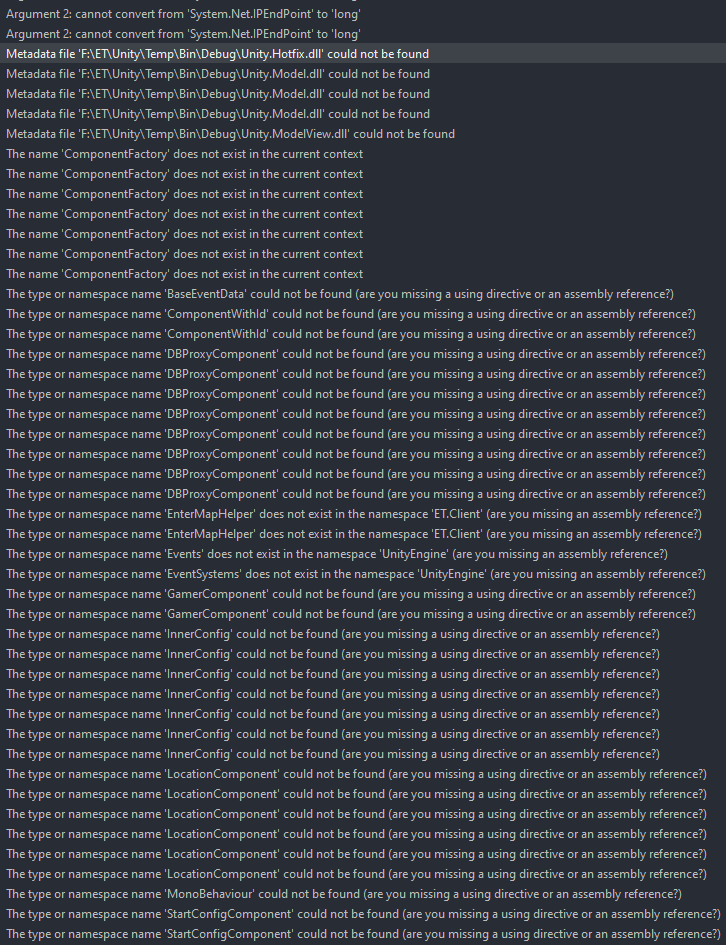
\includegraphics[width=.9\linewidth]{./pic/et4_20230623_152737.png}

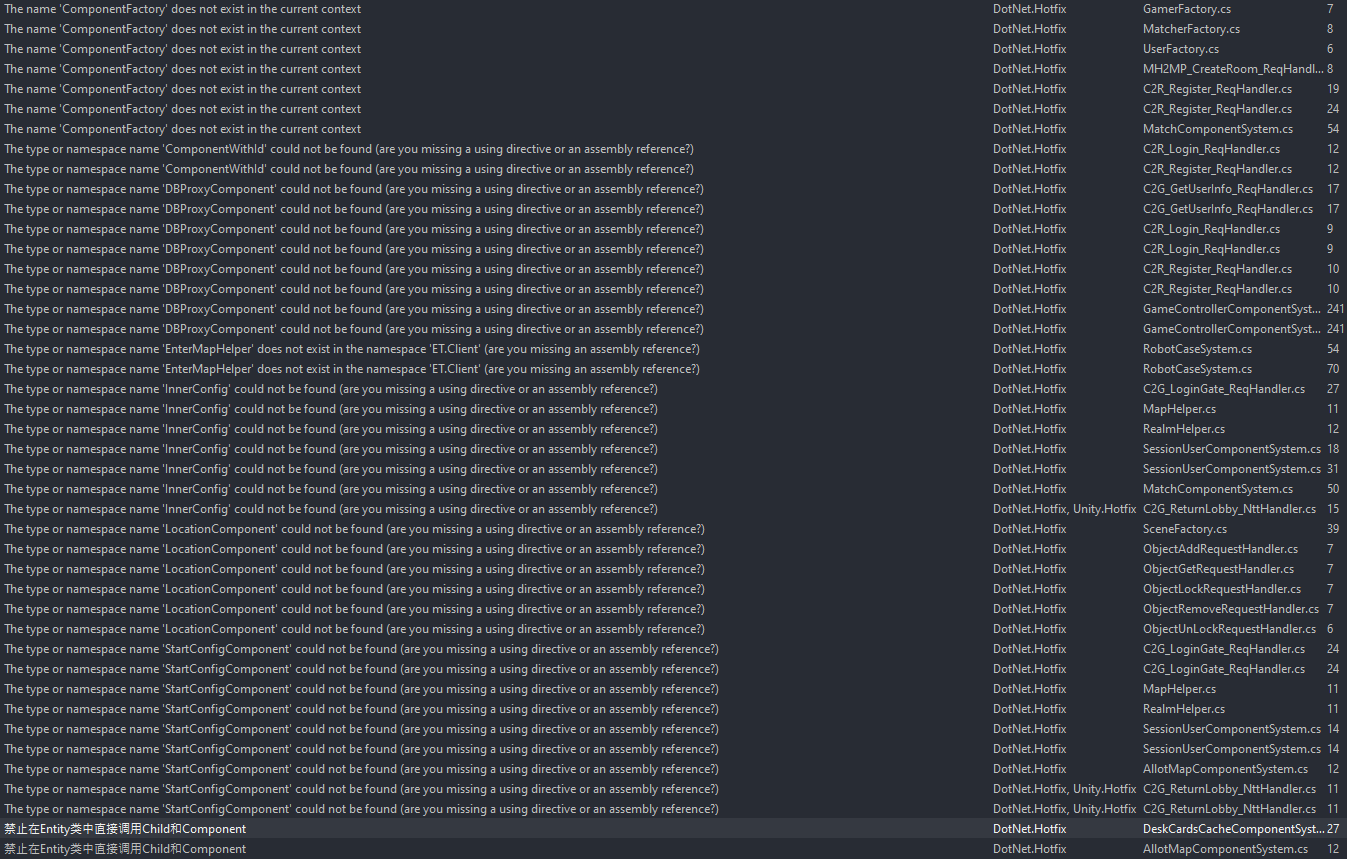
\includegraphics[width=.9\linewidth]{./pic/et4_20230616_165750.png}
\begin{itemize}
\item 【ComponentFactory:】重构了的框架里,这个工厂类是被折解到各自小部件的生产工厂里去了,就是一个框架底层封装的工厂类,拆解到 100 个不同的小部件里。所以我必须得要每个使用的小部件里,它的生产工厂里去再调用相应的逻辑。【可以找个例子出来看一下】
\begin{itemize}
\item Entity 类里面有,组件里添加一个新 new 出来的成员的办法。模仿Player 的使用例子。这里的使用方法是:去拿它的管理组件的实例索引,用管理组件来生成各个元件
\end{itemize}
\item 【PlayerSystem】:不是不知道框架里怎么用,找不出来一个使用的例子吗?它可能不需要用,它只需要框架底层的Entity 里相关方法的封装,能够生成一个一个小单元(Player,Gamer,Matcher-etc)之类的就可以了。就是框架底层原理,这一块儿的,还不太懂
\begin{itemize}
\item 这个工厂类,总是不懂,先去把基类Entity.cs 好好再读一下
\item 同样套用的话,GamerComponent 是房间组件的子组件,拿到这个组件后来创建. VSC 里面好像是有多余的类,所以从 VSC 里看源码,比较乱一点儿。【感觉这一块儿的思路,还没能理清楚。】
\item Hotfix Server \textbf{【UnitFactory】} 生成创建一个单位。可以用作例子。unitComponent.AddChildWithId() 调用的是Entity 里最底封装逻辑。
\begin{itemize}
\item 这个UnitFactory 调用组件方法,来添加进自己的管理系,它所添加的组件是有独特身份ID 的,不适用当前例子
\item 需要去找,自动生成特异性ID, 并创建实例的 Entity 里的方法的例子
\end{itemize}
\item 上面的问题是,如果框架热更新域里可以如上 UnitFactory 一样添加工厂类,那么我的其它小单位Gamer, Player 应该也是可以如上Unit 一样提供他们自己的工厂生产类才对。
\item 再试着多找几个如上的工厂生产类的例子看看。
\end{itemize}
\item \textbf{【ComponentFactory.CreateWithId:】} 重构了的框架里,这个工厂类是被折解到各自小部分的生产工厂里去了,就是一个框架底层封装的工厂类,拆解到 100 个不同的小部件里。所以我必须得要每个使用的小部件里,它的生产工厂里去再调用相应的逻辑。【可以找个例子出来看一下】新框架里,上次不是找到过:先去拿管理器组件,再用管理器组件,通过调用基类Entity 里的方法,来创建小部件的实例?可以再找个例子看一下
\item 上午把【数据库模块的接入】、【InnerConfig】【StartConfigComponent】【LocationComponent】等相关模块:读下源码,理解透彻,必要的情况下下午家里接入并测试
\begin{itemize}
\item 把ActorLocation 相关的,今天晚上一个小时左右,再读一下
\end{itemize}
\item \textbf{【GamerComponent】} :它的逻辑设计应该是什么样的?当服务端有 PlayerComponent 对所有玩家进行管理,当前GamerComponent 只管理一个拖拉机房间里的四个玩家,是RoomComponent 的玩家组成对象(?还有房间组成对象,因为房间如玩家一样需要管理,对应不同拖拉机房间号)$\backslash$
\begin{itemize}
\item 参考项目放在热更新域里面,但是现项目是不允许申明组件放在热更新域里的。去参考项目中其它组件是否全在Model 层申明组件,以及成员变量。暂时把它放到Model 双端共用的地方。
\item 台式机好慢好慢,找了好久才找到这个类。现在应该可以往下改了。这个模块,今天就暂时改到这里,看不见什么相关的编译错误了
\item 这里看出 ET 框架的局限:它把一切成员变量之类的在Model 层里固定死了,也就意味着,热更新是无法热更新功能逻辑模块的重构,只能热更新小细节的实现逻辑。
\end{itemize}
\item \textbf{【GamerComponent 管理类组件】} :逻辑没有理清楚。它是服务端组件,还是客户端组件,还是如PlayerComponent 双端组件,并实现不同的逻辑?
\end{itemize}
\subsection{内网消息等网络相关:请求消息的发送方法等。狠多编译错误,要一点儿一点儿把他们都改掉}
\label{sec-4-3}
\begin{itemize}
\item \textbf{【内网消息等网络相关:请求消息的发送方法等】}: \textbf{在构架里是怎么写的,有几种请求消息的发送方式?}
\item \textbf{明天上午把这块看完,等着我改的编译错误包括} :参考的斗地方游戏里,各种服处理返回消息的逻辑。
\begin{itemize}
\item 因为先前手动发送每个返回消息,我需要将这部分一批消息处理器改为,先试着适配 ET7 框架的重构与底层再封装。
\item 等改过了,真正明白理解了自己重构游戏的需求,再来看去看ET7 框架我要怎么改它现存封装,才能适配自己游戏的需求!!例子:MatchComponentSystem 里的JoinRoom 方法等相关逻辑。
\item 【下午还没有改到这里来。先从简单的改起,因为一个热键的优化,感觉VS 好用一点儿了。先能改多少改多少,再按模块来改像消掉所有的ETTask 相关一样把一个模块的所有的编译错误全部改完!!!】
\end{itemize}
\item 去看上面列过的那个例子MatchComponentSystem, 参考项目里的各种服的消息处理,怎么适配成ET7 重构后的不用手动发返回消息(发送过程封装在框架底层),和记录可能存在的问题(某些服的逻辑,返回消息的发送时间与其它必要逻辑,顺序变得重要的时候,记下来,晚点儿会再重构ET7 框架适配游戏需求)
\end{itemize}
\subsubsection{修改下面的ActorMessageSenderComponent 因为功能模块逻辑重构,而带来的一堆编译错误。}
\label{sec-4-3-1}
\begin{itemize}
\item 修改方法过程步骤:去框架里搜索,其它任何地方发送消息的例子,看 \textbf{【重构后的框架是如何发送消息的, Call() Send() 方法的调用等】} 这个明天上午一定看,因为不懂,不会改怎么发送消息的()
\item 然后参照例子,把客户端和必要的小服里,所有需要发送消息的地方,改成上面看到总结的发送方法里。
\end{itemize}

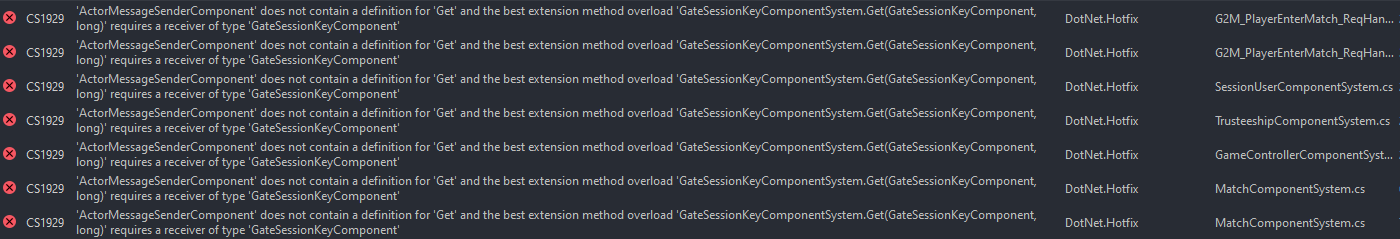
\includegraphics[width=.9\linewidth]{./pic/et4_20230616_160327.png}

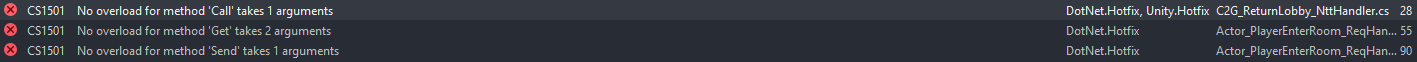
\includegraphics[width=.9\linewidth]{./pic/et4_20230616_165027.png}
\begin{itemize}
\item 【地图服Unit 相关】:先前所有接触到这个框架,都只看了个头,就是只限于能够任何客户端连接到服务端能够注册登录的程度,后面的其它服、框架逻辑全都还不曾看。所以今天上午扫一眼地图服相关,是糊的。要把这些前前后后相关的原理总弄懂了。
\item 去框架里搜发送的调用方法,可能现在 Mac 系统里有一点儿障碍的,就是VSC 不报错,不知道搜出来的是对的,还是错的。但是几种不同的方法,先总结在这里,对照运行时的报错一一改过来。必须把这块儿弄明白了。【爱表哥,爱生活!!!任何时候,活宝妹就是一定要嫁给亲爱的表哥!!爱表哥,爱生活!!!】
\item 【拿到Session 会话框,调用其Send() 方法】:例子 PingComponentAwakeSystem 里的 PingAsync() 方法。它是一个心跳包。这个心跳包就是一Awake() 醒来,全生职责就是周期性给服务器发消息
\item 然后参照例子,把客户端和必要的小服里,所有需要发送消息的地方,改成上面看到总结的发送方法里。
\item 框架里,各种不同场景下发送消息的方法:
\item 【场景里拿到SessionComponent】,调用会话框的发送方法Send()
\begin{minted}[fontsize=\scriptsize,linenos=false]{csharp}
robotScene.GetComponent<Client.SessionComponent>().Session.Send(new C2M_TestRobotCase2() {N = robotScene.Zone});

// 也可以借助UnitGateComponent 拿到它的成员变量 GateSessionActorId, 用这个可以重构后发消息
ActorMessageSenderComponent.Instance.Send(u.Unit.GetComponent<UnitGateComponent>().GateSessionActorId, message);
\end{minted}
\item 【活宝妹任何时候就是一定要嫁给亲爱的表哥!!!】迷迷糊糊地把一个模块改完了,可是感觉那个改掉的模块,像是还没能理解透彻。明天上午会再看一下。【爱表哥,爱生活!!!任何时候,亲爱的表哥的活宝妹,就是一定要嫁给亲爱的表哥!!爱表哥,爱生活!!!】70 Compile Errors 还没有改完,涉及功能模块人接入与整合。会明天上午看过读一下相关模块的源码后再试着改。【活宝妹就是一定要嫁给亲爱的表哥!!!爱表哥,爱生活!!!】
\end{itemize}
\subsubsection{【ActorMessageSenderComponent】:这个类狠重要、狠重要,现在是活宝妹理解网络模块的核心。爱表哥,爱生活!!!}
\label{sec-4-3-2}
\begin{itemize}
\item 得去想:ActorMessageSenderComponent, 是只能用来处理跨进程消息的吗?普通消息的发送是如何处理的?该弄明白,它的适用范围,适用哪些情境上下文
\item \textbf{【ActorMessageSenderComponent】} :因为ET7 这个模块的重构。不再需要每个返回消息手动去拿消息发送器,交由框架底部去处理。
\item 不懂的是,如何重构,消除参考项目里各种服的消息处理里,怎么适配成ET7, 不用去拿消息发送器,只把返回消息结果写好,或是发送(请求)消息时,如何发送?
\item 不同于昨天上午看过的,NetInnerComponentOnReadEvent 是对上层读到消息后的处理,就是消息已经准备好了,甚至已经通过某种逻辑代理,到达和触发了NetInnerComponentOnRead 事件了(这个事件是怎么触发的?大概是,每个进程会有一个内网组件NetInnerComponent. 当内网组件读到消息会触发。读到消息,包括本进程消息,也就包括,由其它进程发回来的返回消息。这个,可能更底层Session 发回来跨进程消息的地方?改天去捡)。现在要去理解的是,比如发送一条请求消息,创建一个请求消息实例后,如果运动可以走到上面的触发读到消息事件?就是消息流程的前半部分。NetInnerComponentSystem.cs 的读到消息事件,要再往前看一点儿。
\item 把消息的处理流程几个重要的方法 \textbf{【ActorMessageSenderComponentSystem Send() Call() 等】} ,这里再梳理一遍:
\end{itemize}
\begin{enumerate}
\item ActorMessageSenderComponentSystem Send():
\label{sec-4-3-2-1}
\begin{itemize}
\item 【任何时候,活宝妹就是一定要嫁给亲爱的表哥!!!活宝妹若是还没能嫁给亲爱的表哥,活宝妹就永远守候在亲爱的表哥的身边!!爱表哥,爱生活!!!】
\item 今天终于把里面的计时器原理看懂了。
\item \textbf{【ActorMessageSenderComponentSystem Send()】} 发的是普通消息(不是不需要回复消息,是任何消息,都走这一步,因为是最基的基类接口)
\begin{itemize}
\item 【同一进程消息】:不走网络层,直接交由本【进程?】的消息处理器处理。就是(ActorMessageSenderComponentSystem Send()里)判断如果是同一进程,它会调用内网组件处理消息:NetInnerComponent.Instance.HandleMessage(actorId, message); 【注意这里是一个进程内网组件消息的一个来源:本进程消息。它同样接收和读来自其它进程的消息,跨进程消息】。而内网组件的这个HandleMessage() 静态方法,就发发布内网组件读到消息事件;内网组件读到消息事件的发布,会触发调用 NetInnerComponentOnReadEvent 借助 ActorHandleHelper 来处理内网消息。后面的就是昨天上午读到的部分。这里的疑问就是:谁,哪里调用发送组件的Send() 发送事件?
\item 【不是同一进程消息】:就通过内网组件,去拿同那个收消息进程的会话框,通过会话框走Session 流程发跨进程消息。就是走网络层。
\end{itemize}
\end{itemize}
\item ActorMessageSenderComponentSystem Call()
\label{sec-4-3-2-2}
\begin{itemize}
\item \textbf{【ActorMessageSenderComponentSystem Call()】} 发的是要求返回结果的消息:返回 ETTask<IActorResponse>
\begin{itemize}
\item 注意 \textbf{【跨进程消息的回复细节里】} ,看见IRpcResponse 实例创建好,结果写好,同步到异步任务ETTask 里,总容易忘记ETTask 的异步任务运行结束(如果不是抛异常), \textbf{跨进程消息是如何回到消息的发送进程的?} 是AMRpcHandler 抽象类里,异步等待实体实现类里的具体实现逻辑Run() 异步方法执行结束,也就是等待各种消息处理服处理好、写好异步返回消息IRpcResponse, 同步到异步任务ETTask. AMRpcHandler 抽象类里等异步方法执行完成,抽象类里作了封装,把返回消息通过进程间通信会话框,把返回消息发回去的。
\item 这里看见,这个消息发送器底层逻辑说,如果是我自己进程要发消息,就封装消息发送者 rpcId 是自已的 rpcId. 然后调用自组件Call() 发送消息。后面的几个方法,大概就是跨进程消息的发送与回复。
\end{itemize}
\end{itemize}
\end{enumerate}
\subsection{静态类的环形引用问题}
\label{sec-4-4}
\begin{itemize}
\item 静态类 CardsHelper, 与静态类 DeskCardsCacheComponent.System 之间,存在静态类的互相引用:就是说,两个静态类,互相引用了对方的方法
\begin{itemize}
\item CardsHelper 里,引用了DeskCardsCacheComponent.System 里的方法
\item 而 DeskCardsCacheComponentSystem 类里,同样引用了 CardsHelper 里的方法
\item 我的解决办法是:热更域里的 DeskCardsCacheComponentSystem 对CardsHelper 类里引用的两个静态方法,直接复制了一份在 DeskCardsCacheComponentSystem 类里面,就可以消除了。再次体验VS 的显著延迟,真让人受不了。是因为这个软件被监控吗?
\end{itemize}
\end{itemize}
\subsection{下面是已经改好了的:还是先放着,备查}
\label{sec-4-5}

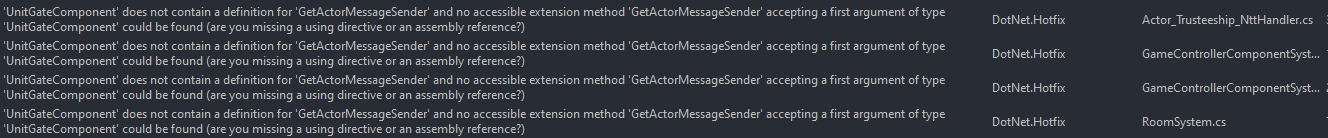
\includegraphics[width=.9\linewidth]{./pic/et4_20230616_162711.png}
\begin{itemize}
\item 【UnitGateComponent]: 怎么才能成为多个不同组件的组成部分?
\end{itemize}

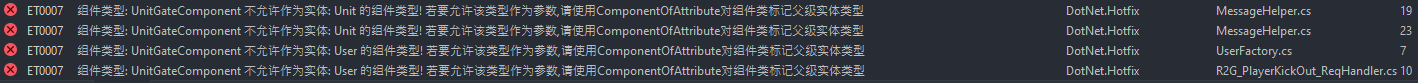
\includegraphics[width=.9\linewidth]{./pic/et4_20230616_165317.png}
\begin{itemize}
\item 【解决办法】:去查框架里的源代码,写得极其清楚:
\begin{minted}[fontsize=\scriptsize,linenos=false]{csharp}
// 组件类父级实体类型约束
// 父级实体类型唯一的 标记指定父级实体类型【ComponentOf(typeof(parentType)】
// 不唯一则标记【ComponentOf]
[AttributeUsage(AttributeTargets.Class)]
public class ComponentOfAttribute : Attribute {
    public Type Type;
    public ComponentOfAttribute(Type type = null) {
        this.Type = type;
    }
}
\end{minted}
\begin{itemize}
\item 所以上面的解决办法就是:不要标记 typeof 参数就可以了呀,它就可以成为多个不同组件的子元件部件了呀。。。是这样的
\end{itemize}
\begin{minted}[fontsize=\scriptsize,linenos=false]{csharp}
[ComponentOf] 
public class UnitGateComponent : Entity, IAwake<long>, ITransfer, ISerializeToEntity { // 不知道这里为什么会受到限制,这里再改一下
    public long GateSessionActorId { get; set; }
    // 想一下,下面的变更还需要吗?要不要,是看框架里有没有什么,自动上线自动下线处理之类的,相关的?
    public bool IsDisconnect;
}
\end{minted}
\end{itemize}
\subsection{先前列的相对杂一点儿}
\label{sec-4-6}
\begin{itemize}
\item 【问题】:上次那个ET-EUI 框架的时候,曾经出现过 opcode 不对应,也就是说,我现在生成的进程间消息,有可能还是会存在服务器码与客户端码不对应,这个完备的框架,这次应该不至于吧?
\item 【UIType】部分类:这个类出现在了三四个不同的程序域,现在重构了,好像添加得不对。要再修改
\item \textbf{【ET7 框架】} 没有处理的逻辑是: \textbf{【ET7 框架里数据库的接入】}
\item \textbf{【UILobbyComponent 可以测试】} :这个大厅组件,Unity 里预设简单,可以试运行一下,看是否完全消除这个UI 组件的报错,这个屏的控件能否显示出来?还是错出得早,这个屏就出不来已经报错了?
\begin{itemize}
\item 【客户端】的逻辑是处理好了,编译全过后可以测试
\item 【服务端】:处理用户请求匹配房间的逻辑,仍在处理: \textbf{C2G\_StartMatch\_ReqHandler}.
\end{itemize}
\item \textbf{【TractorRoomComponent】} :因为是多组件嵌套,可以合并多组件为同一个组件;另早上看得一知半解的一个【ChildOf】标签,可以帮助组件套用吗?再找找理解消化一下
\item 【房间组件】:几个现存的 working-on 的问题:
\begin{itemize}
\item 多组件嵌套:手工合并为一个组件。彻底理解确认后,会合并
\item 【服务端】:处理用户请求匹配房间的逻辑. 这里的编译错误终于改完。到时就看运行时错误了。
\begin{itemize}
\item 【数据库模块的整合】:网关服在转发请求匹配时,验证会话框有效后,验证用户身份时,需要去【用户数据库】拿用户数据。ET7 留了个DBManagerComponent, 还没能整合出这个模块
\end{itemize}
-【参考来源 \textbf{C2R\_LoginHandler} 】:Realm 处理客户端的登录请求的服务端逻辑。这里看见,它随机分配一个网关服。也就是,我(原本本质上也是随机分配)一个匹配服给用。可以依照这里的例子来改写。
\end{itemize}
\item 【匹配服地址】网关服的处理逻辑里,验证完用户合格后,为代为转发消息到匹配服,但需要拿匹配服的地址。ET7 重构里,还没能改出这部分。服务器系统配置初始化时,可以链表管理各小构匹配服,再去拿相关匹配服的地址。ET7 框架里的路由器系统,自己还没有弄懂。
\item \textbf{【ET7 IMHandler 对回复消息的写封装, 与自动回复消息的封装】} :可能无法处理游戏过程中的某些逻辑。就是涉及到一定顺序,尤其需要先回复消息的处理服处理逻辑。举例:C2G\_StartMatch\_ReqHandler. 所以,这里要自己好好想透彻一点儿。要如何改,才能适配自己游戏的需求。
\item \textbf{【 ComponentFactory:】} ET7 里重构,被分布到各种不同的组件里去了。想复制个文件过来,把与之相关的全部消掉,但因为大规模重构,复制了文件也没用。总之ET7 就是感觉什么乱七八糟的,感觉他们大规模糊乱重构的目的就是故意挫败人。可是这个世界上就偏偏存在亲爱的表哥的活宝妹这样的不服的!!!爱表哥,爱生活!!!任何时候,活宝妹就是一定要嫁给亲爱的表哥!!!爱表哥,爱生活!!!

\item \textbf{【PlayerComponent 类重复】} : 狠奇怪:删除了说找不到类,不删除说重复了,感觉台式机应用有延迟?反应狠慢。。。。。文件嵌套想要显示所有嵌套文件的时候,要狠久狠久重启好几次才反应得过来
\begin{itemize}
\item 原本有两个类都是如上面这个类这样,但有时候台式机反应稍快一点儿,就是一个类找不到出现上面的情况。破电脑的延迟反应,弄得我都要怀疑VS 应用被别人操控了。。。
\item 【爱表哥,爱生活!!!任何时候,活宝妹就是一定要嫁给亲爱的表哥!!!爱表哥,爱生活!!!】
\end{itemize}
\item 把还没有用到,但是报错了的几个类删掉:比如记一下: SessionInfoComponent,
\begin{itemize}
\item 还剩最后 26 个最挑战活宝妹的编译错误,今天傍晚会家里改会儿,集中问题明天上午希望能够看懂。【爱表哥,爱生活!!!任何时候,活宝妹就是一定要嫁给亲爱的表哥!!】
\end{itemize}
\end{itemize}

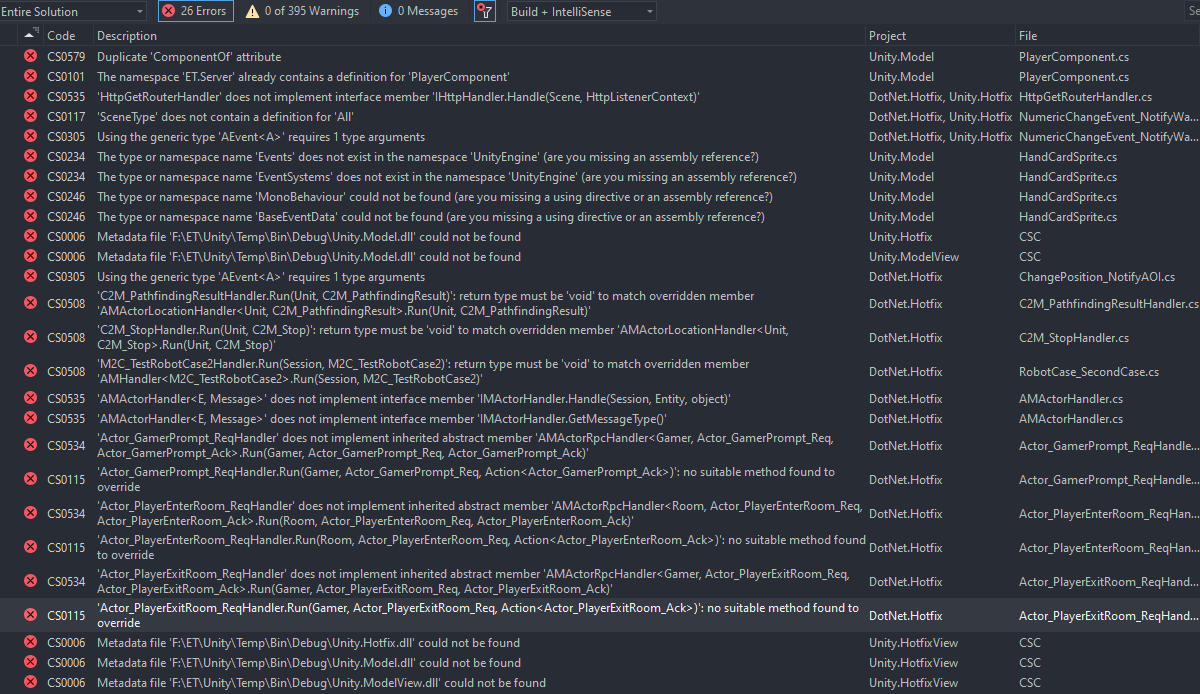
\includegraphics[width=.9\linewidth]{./pic/et4_20230604_162732.png}
\begin{itemize}
\item 把Root 根场景以及启动时添加的组件大致看了一遍。想把上面的消息处理器再系统化地看一遍,理解一下,总改不到这个模块相关的编译错误。
\item \textbf{【ETTask ETVoid 是必须弄懂的】} ;看两个小时,像昨天晚上一样真正投入进去看。我相信自己看得懂,弄得透,只是需要投入一点儿时间。
\begin{itemize}
\item 感觉前一个周左右的时间,倍受睡眠困扰。活宝妹做梦也不会想到,昨天的自己会困成那个样子(感觉开1 小时的车极度困难,太容易睡着。。)。。现在试着一再调整状态,少喝咖啡多运动,最重要的,仍是把学习的状态调整出来调整回来。至少学到活宝妹可以嫁给亲爱的表哥的这一天!!!
\item 这个异步的原理,感觉是弄明白了,今天上午又看了一遍看了会儿。下午去改那些 IMHandler, 希望今天下午能够改彻底。就是真正弄明白了去改(现在的问题就是,几个IMHandler 的实体实现类,改天这个顾不了那个,没弄明白,接口方法怎么申明定义,才能兼顾所有实例类消息处理器?),不是只改掉了当前的编译错误,等真正运行的时候,一个个运行错误或是异常往外冒!!!今天脑袋还算清醒,下午好好弄弄这个
\end{itemize}
\item 【爱表哥,爱生活!!!任何时候,亲爱的表哥的活宝妹,都是一定要嫁给亲爱的表哥的!!!】【三楼上的贱鸡贱畜牲真多!!!一天到底没想点儿好的】活宝妹还没能嫁给亲爱的表哥,活宝妹就是永远守候在亲爱的表哥的身边!!!爱表哥,爱生活!!!
\item 再然后 ,再看下下面的 UnitGateComponent 相关。下午或傍晚有时间的时候,可以再折腾折腾 emacs-org-mode 下划线删除字体设置为斜体。
\item \textbf{【UnitGateComponent】} 加个方法用?可能不需要加方法;另一个错是,不能同时成为两个不同 entity 的子控件?【ComponentOf(typeof(Unit))】etc 出错文件在 (C2G\_EnterMapHandler)
\begin{itemize}
\item 这里要把 ActorMessageSenderComponent 组件给弄明白。它有个有序管理字典,记着 actorId 与ActorMessageSender 的一一对应关系,就可以封装维护消息的自动发送等,以及必要的超时消息管理。
\end{itemize}
\item \textbf{【服务端Actor\_PlayerEnterRoom\_ReqHandler 这个处理类】} 现在还很多问题,需要弄懂,往下改
\item 今天晚上会把刚才下午看见、意识到几个模块的问题试着分析明白,记下笔记。
\item \textbf{ETTask-vs-ETVoid}: 框架里有狠多需要改的地方。今天上午的脑袋好使,把这块儿再仔细好好看下。今天上午把以前不懂的模块都稍微看下,再理解一下
\begin{itemize}
\item 查网页感觉也查不出什么来。还是用源码帮助理解概念。【爱表哥,爱生活!!!活宝妹就是一定要嫁给亲爱的表哥!!!】
\item 不能把所有基类的 async ETTask 返回参数直接改成 void, 因为框架的顶层应用,服务端或是客户端,当不异步等待结果,如资源包没能下载完成,就接着往下执行,会报空异常。
\end{itemize}
\item 现在的问题是:Protobuf 里 repeated 关键字,好像还是没有处理好,找不到成员变量  Cards. 是因为 Proto2CS 的时候,确实把 repeated 关键字给处理丢了。因为我的 .proto 文件里有错误。(这就是上面先前觉得奇怪的原因。因为改这个的过程中把那些错改正了,就可以生成成功并找到相关的消息了)。
\item 这部分总感觉弄得不是狠透彻。就再花点儿时间。这段时间产量太低,可以先试着完成其它模块。
\item \textbf{【HandCardSprite 这个最近要弄明白】} 不知道这个类是为什么,整了一堆的错误,它是ETModel 里的。感觉是常规域,没弄明白为什么常规域还有ILRuntime 的适配呢?
\begin{itemize}
\item 要把 ILRuntime 热更新第三库,也再弄得明白一点儿【今天上午把这里再看,最好是能够结合源码看看】为什么这个类还要适配ILRuntime ?
\item 这里这个类,整个框架里只找到这一个用的地方,所以它一定是添加在某个预设或是场景中的某个控件下的。只是参考项目的unity 客户端,我运行不到打牌的这个界面,就先因为抛出异常而淡能运行。所以还没能找到哪个预设或是场景中的哪个控件添加了这个类,但是当然一定是跟玩家手牌相关的。 \textbf{【HandCardSprite 是在 handcard 预设里添加了这个脚本】}
\item 这个类今天运行狠奇怪,VS022 里找不到了。。。就是说,VSC 里它是在Model 客户端的源码里,但是从VS 里打开,找不到这个类文件所在的文件夹和文件,没有索引好,再添加一下?
\item 那么,为什么前两天被这个 block 住,而那天,好像是有删除掉这个文件,但文件夹应该是还在的才对呀?我可能还会试着再把它添加回去。
\item 但是,会在把当前几个编译错误改完,试着测试一下客户端现在有的界面之后,再试着添加回去,整理和 develop TractorRoomComponent 界面的内容。【爱表哥,爱生活!!!活宝妹任何时候就是一定要嫁给亲爱的表哥!!】
\item 今天下午家里再运行一次,当客户端抛异常,应该是某个热更新的资源包没有找到什么的?所以可以试着自己去解决这个客户端实时运行时抛出的异常。
\item \textbf{【参考项目斗地主客户端异常】} :再运行一次,试着分析,是否可以 unity 里实时运行,如果不可以,为什么不可以?
\begin{itemize}
\item 应该是LandlordsRom 这个预设与UI 类型没能连接起来,也就是找不到这个预设。
\item 那为什么打好包的可以呢?因为打好包的预设包名 LandlordsRoom.unity3d 与游戏逻辑契合,可以找得到
\item 可是仍然感觉奇怪:LandlordsLogin 与LandlordsLobby, 非常类似都可以找到,为什么就LandlordsRoom 找不到?可能LandlordsRoom 预设还是有某点儿物对特殊的地方。
\item 上面这个暂时跳过。现在仍然主要去看HandCardSprite 为什么参考项目里可以,而ET7 里就不可以。
\end{itemize}
\item 就是上面那个异常,今天下午得去弄明白,为什么只在 unity 实时运行时会抛异常,而如果是三个打包好的客户端,就不会。也就是说,打包好的不存在找不到类、找不到预设、或是找不到任何相关资源的问题。
\item 这个项目Unity.Model 是需要索引 UnityEngine 以及UI 等相关模块人的 .dll 的。暂时还没弄明白它是怎么加的
\item 【爱表哥,爱生活!!!任何时候,活宝妹就是一定要嫁给亲爱的表哥!!】
\end{itemize}
\item \textbf{ClientComponent} 参考项目组件:去看ET7 里客户端的 PlayerComponent.
\item 【爱表哥,爱生活!!!任何时候,活宝妹就是一定要嫁给亲爱的表哥!!!】今天下午先去看 Tractor 游戏源码,设计重构思路
\item 【活宝妹坐等亲爱的表哥,领娶活宝妹回家!爱表哥,爱生活!!!】
\item \textbf{【亲爱的表哥,这个世界上,只有一个活宝妹,这么心心恋恋,就是一定要嫁给亲爱的表哥!!!问世间情为何物,直教人生死相许。。亲爱的表哥,一个温暖的怀抱拥抱的魂力可真大呀,管了这如许多年!!这不,你的活宝妹为了这个温暖的怀抱拥抱,就是一定要嫁给亲爱的表哥!!不嫁就永远守候在亲爱的表哥的身边!!爱表哥,爱生活!!!活宝妹就是一定要嫁给亲爱的表哥!!!】}
\item 亲爱的表哥,活宝妹相信舅舅十岁闯江湖的阅历,活宝妹深深相信亲爱的表哥。活宝妹就是稳稳地永远守候在亲爱的表哥的身边!爱表哥,爱生活!!!活宝妹就是一定要嫁给亲爱的表哥!!
\item 【爱表哥,爱生活!!!任何时候,活宝妹就是一定要嫁给亲爱的表哥!!!】
\end{itemize}
\subsection{LocationComponent: 【任何时候,亲爱的表哥的活宝妹就是一定要嫁给亲爱的表哥!!!爱表哥,爱生活!!!】}
\label{sec-4-7}
\begin{itemize}
\item 【今天上午】:从这里开始,把先前总结 Actor 消息以及处理器时,所有关于位置的消息,以及相关的消息处理器弄懂。【没看完】
\begin{itemize}
\item 先前,消息处理器的部分,只看了一个接口类和两个抽象实现,其它没看
\item 消息,位置消息相关的内容,还没看不懂。
\end{itemize}
\item 【亲爱的表哥,活宝妹一定要嫁的亲爱的表哥!!任何时候,活宝妹就是一定要嫁给亲爱的表哥!!爱表哥,爱生活!!!】
\item 【任何时候,亲爱的表哥的活宝妹,就是一定要嫁给亲爱的表哥!!!爱表哥,爱生活!!!】任何时候,活宝妹还没能嫁给亲爱的表哥,他们就大可不必发疯犯贱。任何时候,他们发疯犯贱,他们也永远只能是发疯犯贱得了一时,发疯犯贱不了一世。亲爱的表哥的活宝妹,若是还没能嫁给亲爱的表哥,亲爱的表哥的活宝妹,就是永远守候在亲爱的表哥的身边!!爱表哥,爱生活!!!
\item 因为框架狠大,是一个大型网络游戏双端框架,因为内容比较多,现在已经总结的是四个文件,还要常作笔记,否则容易忘记,前后不连贯。所以难免小细节的地方,没能注意到,没什么大不了
\item 这个模块的编译错误,被活宝妹全部给消除掉了。。。
\end{itemize}
\subsection{【数据库模块:】:这个模块的编译错误,昨天下午清理完了}
\label{sec-4-8}
\begin{itemize}
\item DBProxyComponent: 这个类被重构丢了。数据库分区管理。根据用户所在的区号,去拿该区数据库索引办事就可以了。
\item DBManagerComponent: 全框架找不到一个使用的样例。我认为数据库应该只属于服务端。所以,我先把它在应用启动时添加到服务端的公用组件启动程序中(EntryEvent2\_InitServer)去。
\item 下午把几个DBProxyComponent 相关的编译错误,基本改光了(目前还有几个小模块共计28 个编译错误)。还有一个类里不知道怎么用Gamer 去拿玩家所在的小区,先放一下,改天再去改个。
\item 【任何时候,活宝妹就是一定要嫁给亲爱的表哥!!!】
\end{itemize}
\subsection{【HandCardSprite.cs】}
\label{sec-4-9}
\begin{itemize}
\item \textbf{【HandCardSprite.cs】} :这个客户端文件里存在一堆关于Unity 引用的错误。把这个有着巨多错误的类重新添加到了框架里。现在着眼着这些错误(加了这个文件,错误又多了二三十个!!!)。
\begin{itemize}
\item \textbf{【参考项目Game.cs】} 客户端类里,存在UnityEngineer 的诸多引用,所以HandCardSprite.cs 可以通过Game.EventSystem 等拿到引用。但ET7 重构得没有边际。必须自己去看明白。这个类,更多的是,适配特定游戏需求的ET7 框架外的一个桥梁适配类。
\item 【参考项目热更域里的 Game.cs 类】:
\begin{minted}[fontsize=\scriptsize,linenos=false]{csharp}
public static class Game {
    private static Scene scene;
    public static Scene Scene {
        get {
            if (scene != null) 
                return scene;
            scene = new Scene();
            return scene;
        }
    }
    private static EventSystem eventSystem; // <<<<<<<<<<<<<<<<<<<< 
    public static EventSystem EventSystem {
        get {
            return eventSystem ?? (eventSystem = new EventSystem());
        }
    }
    private static ObjectPool objectPool; // <<<<<<<<<<<<<<<<<<<< 
    public static ObjectPool ObjectPool {
        get {
            return objectPool ?? (objectPool = new ObjectPool());
        }
    }
    public static void Close() {
        scene.Dispose();
        scene = null;
        eventSystem = null;
        objectPool = null;
    }
}
\end{minted}
\end{itemize}
\item 现框架里不存在的,需要整合进来的模块版块:DBProxyComponent, InnerConfig, LocationComponent, StartConfigComponent
\item 组件管理类:某些组件,属于双端,但客户端与服务端的逻辑不一样,如PlayerComponent; 某些组件,只属于服务端;有只属于客户端的吗?
\end{itemize}
\subsection{三件杂事:【任何时候,亲爱的表哥的活宝妹就是一定要、一定会嫁给活宝妹的亲爱的表哥!!!爱表哥,爱生活!!!】}
\label{sec-4-10}
\begin{itemize}
\item 【先花 10 分钟左右,搜下看 emacs-export-to-pdf 与 Skim 应用的自动同步,能理解回调适配过程吗?】还是比较麻烦,改天傍晚或是晚上再凭兴趣来解决,早上看别的
\begin{itemize}
\item 这里主要的问题时,Skim 实时更新外源 pdf 的更新时,因为 emacs 的 export-to-pdf 有个过程,这个过程中生成 table-of-contents 比较靠后,如果不背便条,就必须得每次重点查看TOC. \textbf{Skim 怎么才能够接收到 latex 生成TOC 完成后的回调,来从 Skim 中显示 TOC?}
\item 这里要去想,为什么背个便条,就能最终自动显示 TOC 了呢?背便条能够最终显示 TOC 是为什么, \textbf{背便条背后的原理,能否借用} ?
\item 另外,【可以考虑, \textbf{过滤掉或是配置掉背便条自动同步过程中的确认窗口繁琐过程} 】如果每个 pdf 的自动生成与刷新,我不需要多次点 enter 确认窗口,我只需要点击一个,或者甚至一个也不需要点,就也算满足用户需求。
\end{itemize}
\item VSC 的配置可能哪里写得不对。以前没有这个问题。现VSC 跳转至 emacs 打开当前 buffer, 不能精确定位到 VSC 中当前 buffer 所在的行。改天有机会的时候再 debug 一下。
\item \textbf{【Mac 系统上的五笔输入、emacs pyim 下的词库管理】} :这个是最让人头痛的,因为不懂,网上能够搜到的千篇一律的都是手动搬输入法里如自己现在这样自带的,无法实时热更新的词库。自己想要实现实时动态构建 librime.1.dylib, 却又还建不出来,尤其想要Mac 下建成功才好用。
\begin{itemize}
\item 例子【会话框】,想要去掉不想要的词库,如【停柩】
\item 明明系统输入法里已经将【停柩】清空了,并Deploy 了重新加载了
\item 明明 .emacs-pyim 已经将它【停柩】清空了,并 pyim-restatrt 了重新加载了
\item 可是输入的时候,【停柩】仍然会一再崩出来干扰,没想明白为什么。我记得自己之前能够把不想要的词库清易清除掉
\item 还存在可能性的话:就是 \textbf{【系统输入法构建的第三方库,被 .emacs 引用,这个第三方库可能没有手动再次构建和更新】} ,所以老词库总是存在烦人。
\item 上午快中午也有简单试一下:问题是,我放入 \textbf{/usr/local/lib 的是 rime 自带的缺省构建库} ,也就是说没有自己修改过词库的更新;我 \textbf{再次构建 emacs 所用到的 liberime.so 同样引用缺省的 rime 自带的缺省构建库} ,同样没有修改过后的词库与更新,所以没能从本质上更新词库。 \textbf{【问题是:全中文网络上下,基本全都是用缺省的库,自已手动动态创建的极少极少。。。】} 可怜的亲爱的表哥的活宝妹宝宝,一定想要手动去折腾这个该死的东西。。。。。
\item 我必须得,自己 \textbf{构建自己手动修改了词库之后的Rime-dylib 第三方引用库给 emacs 用} ,才能把词库改过来。下午看看这个,免得睡着了。。
\item 【爱表哥,爱生活!!!任何时候,亲爱的表哥的活宝妹就是一定要嫁给亲爱的表哥!!爱表哥,爱生活!!!】
\end{itemize}
\item \textbf{【VS 自动跳转Emacs 中打开当前 buffer】}: 我记得上次两个电脑对照,我已经解决了这个问题,从VS 中是可以实现C-c i 跳转到 emacs 中打开VS 中当前 buffer 的。怎么过段时间,这个便利功能又丢了,不能用了?
\begin{itemize}
\item 到亲爱的表哥的活宝妹想要好好改改项目,能够真正 debug 的时候,这些原本便利的功能居然出出错作怪,笔记本打开,再弄一次。我居然忘记了上次我是如何实现这个功能的?我忘记这里当初是怎么实现的了,今天晚上晚些时候,再来调整这些其它功能。【现在暂时就仍然点菜单好了】忍一晚上晚点儿再弄
\end{itemize}
\end{itemize}
\subsection{StartConfigComponent: 现框架里有重构了的版本,在理解现ET7 框架的基础上进行必要适配:先把之前总结的再熟悉一下,下午有时间也看看这个}
\label{sec-4-11}
\begin{itemize}
\item 下面是两个重复了的消息,需要删除掉:
\begin{itemize}
\item C2G\_LoginGate\_Req ==》 C2G\_LoginGate 这些重复的消息,我还没有删除掉。改天最后整理清理源码的时候一起再删除
\item G2C\_LoginGate\_Ack ==》 G2C\_LoginGate
\end{itemize}
\item 这里拿《NetInnerComponent》的方法可以参照:
\begin{minted}[fontsize=\scriptsize,linenos=false]{csharp}
Root.Instance.Scene.AddComponent<NetInnerComponent, IPEndPoint>(processConfig.InnerIPPort);
Root.Instance.Scene.AddComponent<NetInnerComponent, IPEndPoint>(NetworkHelper.ToIPEndPoint($"{startMachineConfig.InnerIP}:{startMachineConfig.WatcherPort}"));
\end{minted}
\item InnerConfig: 可以把老版本里的 InnerConfig 类,参考对比ET7 里的ConfigSingleton<T> 泛型类,来试着理解和适配这相模块。因为同属配置类,就是分两个模块。
\item 今天上午再继续看一模块。把昨天下午感觉有点儿不熟悉的:服务端如何管理随机分配给各客户端的各小服的编号等,以及客户端什么时候、如何进入地图服的弄明白。
\item 因为上午头脑相对清醒,把遇见的凡不明白的模块,都试图理解透彻弄明白,比较RouterAddressComponent
\item 【地图服Map 服】:在整理MapHelper.cs 的逻辑的时候,因为游戏的这块儿逻辑不够熟悉,具体原理,或说是连接过程仍然不是狠懂。
\item 去想的话,感觉当用户注册或是登录帐户的时候,是随机分配一个网关服;框架里也随机分配给用户一个 Realm 注册登录服;当用户点击进入地图,或是重构游戏开始游戏的某个地方,是需要与地图服建立起连接的,大概如果有多个地图服,又随机分配一个。。框架里,虽然分配给每个用户的各个小服,是完全随机的,但是一旦分配给一个用户,除非用户登出下线、或是用户掉线,或是用户其它客户端顶号(用其它客户端的登录顶掉先前某个客户端的登录?这里先前分配的,会变吗?再读的时候看下这块儿),分配给用户的这些小服编号是可能会变的,与先前不同。但同户的同一个玩耍 session ,应该是保持不变的。所以,框架里应该是有某些组件,是可以记录这些小服编号的。要找出来。
\item 感觉我还是需要回去再读一下参考项目斗地主游戏里进入地图服的这块儿逻辑。当地图服要给某个用户发消息,MapHelper 这里的作用,应该就是帮助地图服找到有当前用户所在的网关服会话框,以便地图服向用户所在的网关服发消息。可是,感觉起来,地图服与网关服之间,不该是内网组件去管理吗?如果内网组件能够管理,MapHelper 就显得多余了呀。要去检查的还有RealmHelper. 这里感觉没能理解透彻为什么ET7 要把一个个好多个弄成帮助类。
\item 【活宝妹就是一定要嫁给亲爱的表哥!!!爱表哥,爱生活!!!】
\item 感觉我对源码的管理做得不够好。过程中为什么有很多类,过程中都没能看见呢?为什么分支里明明是有LocationComponent 类,而我先前找不到?
\item 【今天下午】:
\begin{itemize}
\item 因为昨天读【路由器相关模块】,读得感觉比较懂一点儿了。今天下午所所有网络相关的模块再读一遍,什么时候添加的组件,事件的传递顺序等,都弄明白。修改补好笔记。
\item 今天下午会手洗半小时内衣,骑行内衣傍晚会穿出去骑约1-1.5 小时。下午可能会花半小时左右手工。
\item 今天下午家里用大显示器,会希望再读至少 2.5 小时框架里的网络模块,把上午弄得半头三桩,羞于提交上 github 的笔记事理好。
\end{itemize}
\item 【这几天两三天看异步作务异步共享资源锁】:基本把框架里的锁、协程锁,与ETTask 基本上全看懂了。【爱表哥,爱生活!!!任何时候,亲爱的表哥的活宝妹就是一定要、一定会嫁给活宝妹的亲爱的表哥!!!爱表哥,爱生活!!!】
\item 现在就是,接着去看,先前看时,曾经感觉有困难的,参照上面的学习方法,不懂的网络上搜,走到自己把这些先前不太懂的模块都看懂看明白。【爱表哥,爱生活!!!任何时候,亲爱的表哥的活宝妹就是一定要、一定会嫁给活宝妹的亲爱的表哥!!!爱表哥,爱生活!!!】
\item 【亲爱的表哥,现在是,一年中活宝妹的本尊(狮子月)!!】这个月,从今天晚上开始,活宝妹都要尽力好好学习了!!一年 12 个月,只有活宝妹的狮子月,活宝妹的理解力、学习效率最高!!!订个小计划:(看完了【协程锁】与【异步任务】)
\begin{itemize}
\item 搬家前的五天,把框架,如读【协程锁】如读今天晚上,以前看不懂的地方【网络模块】【Actor 模块】【Handler?】【动态路由模块】今晚能懂般,把它们都看懂,作好笔记;
\item 周日周一尽量只下午傍晚去搬,两个下午三四次应该能够搬完。上午和晚上的时间,仍然需要好好学习
\item 8/1/2023: 搬家后,需要尽快适应新环境,找到早上尽早来到学校后,傍晚才回家的午餐不致病健康午餐饮食。如果每天一定需要呆家里一会儿,尽量留在晚上,傍晚弄点儿吃的,晚上家里再学习会儿,保障白天呆学校
\item 下午家里条件也方便,就把框架里的源码能爬多少爬多少出来。。【爱表哥,爱生活!!!任何时候,亲爱的表哥的活宝妹就是一定要嫁给亲爱的表哥!!爱表哥,爱生活!!!】
\end{itemize}
\item 【爱表哥,爱生活!!!任何时候,亲爱的表哥的活宝妹就是一定要嫁给亲爱的表哥!!爱表哥,爱生活!!!】
\item 早上读NetService.cs 里面异步线程三主要回调同步到主线程,感觉仍然读得昏昏的,要再读一遍,找下是哪里调用的。破车昨晚没补好,今天走回家。。【爱表哥,爱生活!!!任何时候,亲爱的表哥的活宝妹就是一定要嫁给亲爱的表哥!!爱表哥,爱生活!!!】
\item 好多天没有回来改这个了。今天下午出去取材料前在大约半小时,能改一个模块最好,改不完一个模块,能改几个错就改几个错。结果改了一处某个地方的,不过其它的都可以再参考今天改的这个,已经有两个例子了:C2G\_ReturnLobby\_NttHandler 和另外一个例子。【爱表哥,爱生活!!!任何时候,亲爱的表哥的活宝妹,就是一定要嫁给亲爱的表哥!!爱表哥,爱生活!
\end{itemize}


\section{位置服LocationComponent 组件:}
\label{sec-5}
\subsection{LocationComponent:}
\label{sec-5-1}
\begin{minted}[fontsize=\scriptsize,linenos=false]{csharp}
namespace ET.Server {
// 这个【ActorLocation】文件夹:原本只是没有ActorLocationSenderOneType.cs 类。不曾细看【跨进程位置】相关
// 【爱表哥,爱生活!!!任何时候,亲爱的表哥的活宝妹就是一定要、一定会嫁给活宝妹的亲爱的表哥!!!爱表哥,爱生活!!!】
    [ChildOf(typeof(LocationComponent))] // 【位置服】的组件:
    public class LockInfo: Entity, IAwake<long, CoroutineLock>, IDestroy { // 打包:协程锁的实例标记号 + 独占锁
    public long LockInstanceId;
    public CoroutineLock CoroutineLock;
    }
    [ComponentOf(typeof(Scene))]
    // 【位置组件】:去细看两个字典,所做的具体的事情。这里是,被自己弄丢了文件,还是自己添加了这个位置服,但是没整合生成系?去看源码,有没有【位置组件】,有没有相应的生成系
    // 没整合生成系:就是这里Model 域里定义了说有个【位置管理组件】,但是热更域里什么也没有,没有定义执行逻辑,需要一个LocationComponentSystem|Helper 之类的类
    public class LocationComponent: Entity, IAwake { 
        public readonly Dictionary<long, long> locations = new Dictionary<long, long>();
        public readonly Dictionary<long, LockInfo> lockInfos = new Dictionary<long, LockInfo>();
        }
    }
}
\end{minted}
\subsection{LocationComponentSystem: 源码里是有这个文件的}
\label{sec-5-2}
\begin{itemize}
\item 几个最主要的方法,看起来狠简单。
\item 两处:【异步返回类型】感觉相对生疏。
\end{itemize}
\begin{minted}[fontsize=\scriptsize,linenos=false]{csharp}
[FriendOf(typeof(LocationComponent))]
[FriendOf(typeof(LockInfo))]
public static class LocationComponentSystem {
// 添加【注册】的是:【被锁 actorId, 当前——独占锁的实例标记号】这里好像被我写错了,值,应该是,被查小伙伴所在进程的地址
    public static async ETTask Add(this LocationComponent self, long key, long instanceId) { 
        using (await CoroutineLockComponent.Instance.Wait(CoroutineLockType.Location, key)) {
            self.locations[key] = instanceId;
            Log.Info($"location add key: {key} instanceId: {instanceId}");
        }
    }
    // 【下线销号移除】:
    public static async ETTask Remove(this LocationComponent self, long key) {
        using (await CoroutineLockComponent.Instance.Wait(CoroutineLockType.Location, key)) {
            self.locations.Remove(key);
            Log.Info($"location remove key: {key}");
        }
    }
    // 【小伙伴云游】:上报、预报上锁时长,可以更长,因为没玩够还是继续被上锁,同一把锁;直到再上报解锁
    public static async ETTask Lock(this LocationComponent self, long key, long instanceId, int time = 0) { // 忘记这个Key 是什么了,是 actorId
        // 【入队列站列排号】:直到获得异步资源,标记是拿到一把【独占锁】
        CoroutineLock coroutineLock = await CoroutineLockComponent.Instance.Wait(CoroutineLockType.Location, key);
        LockInfo lockInfo = self.AddChild<LockInfo, long, CoroutineLock>(instanceId, coroutineLock);
        self.lockInfos.Add(key, lockInfo); // 再封装:【被锁 actorId, lock 结构体】,封装的是真正实时正在锁着的时长、过程
        Log.Info($"location lock key: {key} instanceId: {instanceId}");
        if (time > 0) { // 要求:不立即上锁,给点儿缓冲时间 
            async ETTask TimeWaitAsync() { // 这里没懂:怎么还有个 ETTask 返回类型呢?  // <<<<<<<<<<<<<<<<<<<< 
                long lockInfoInstanceId = lockInfo.InstanceId; // 先记下:当前被锁资源【独占锁】的实例标记号
// 【异步等待】:被要求的时长。它返回【ETTask】类型 ==》这里可以决定这个内部局部异步方法的返回类型吗?
                await TimerComponent.Instance.WaitAsync(time); 
                if (lockInfo.InstanceId != lockInfoInstanceId) // 再检查:独占锁的实例标记号,是否变了?什么情况下,有可能会变呢?
                    return;
                Log.Info($"location timeout unlock key: {key} instanceId: {instanceId} newInstanceId: {instanceId}");
                self.UnLock(key, instanceId, instanceId);
            }
            TimeWaitAsync().Coroutine();
        }
    }
    public static void UnLock(this LocationComponent self, long key, long oldInstanceId, long newInstanceId) { // 解锁
        if (!self.lockInfos.TryGetValue(key, out LockInfo lockInfo)) { // 先检查几个异常
            Log.Error($"location unlock not found key: {key} {oldInstanceId}");
            return;
        }
        if (oldInstanceId != lockInfo.LockInstanceId) {
            Log.Error($"location unlock oldInstanceId is different: {key} {oldInstanceId}");
            return;
        }
        Log.Info($"location unlock key: {key} instanceId: {oldInstanceId} newInstanceId: {newInstanceId}");
        self.locations[key] = newInstanceId; // 写入小本:【被锁 actorId, 当前锁实例标记号】
        self.lockInfos.Remove(key); // 先从字典管理中移除 
        // 解锁:就是回收掉了呀
        lockInfo.Dispose();
    }
    // 这些异步返回类型,看着还理解不太顺。。。
    public static async ETTask<long> Get(this LocationComponent self, long key) { // 查询:位置信息  // <<<<<<<<<<<<<<<<<<<< 
        using (await CoroutineLockComponent.Instance.Wait(CoroutineLockType.Location, key)) { // 挂号排队站队锁:这个步骤,是【异步】
            self.locations.TryGetValue(key, out long instanceId);
            Log.Info($"location get key: {key} instanceId: {instanceId}");
            return instanceId; // 返回 ETTask<lomg> 因为被排队挂号异步等待过
        }
    }
}
\end{minted}
\subsection{LocationProxyComponent:}
\label{sec-5-3}
\begin{itemize}
\item 不知道我先前对【SceneType.Process】的理解与定义,是否正确?:感觉它像是一台物理机N 个核中每个进程上【1-M】个场景中最特殊的一个场景【SceneType.Process】。亲爱的表哥的活宝妹,把它理解成了:同一进程中多线程环境中的主线程。主线程一定存在,每个核都会有一个【SceneType.Process】场景;主线程要同步异步线程结果等,所以这个场景极为特殊。不知道对了没?
\item 这里以一个核一个进程为单位。它是添加在每个进程上【SceneType.Process】,因为其特殊性,可供可代理【1-N】个场景需求与使用?
\item 是【SceneType.Process】层面上添加了这个代理组件。去想, N 台物理机,每台M 个核,共N × M 个进程代理,与N × M 中某一个进程下(可能有的【1-X】个不同场景不同小服中)的一条线程场景【SceneType.Location】【位置服】,与共N × M 个进程代理,之间的链接。
\end{itemize}
\begin{minted}[fontsize=\scriptsize,linenos=false]{csharp}
[ComponentOf(typeof(Scene))] // 每个场景上?,有个位置服代理?每个进程上,有个位置服,想起来应该也是合理的,再检查一下
public class LocationProxyComponent: Entity, IAwake, IDestroy {
    [StaticField]
    public static LocationProxyComponent Instance; // 每个场景上,一个实例
}
\end{minted}
\subsection{LocationProxyComponentSystem:}
\label{sec-5-4}
\begin{itemize}
\item 现在做的事情是:在确认【位置服】位置组件正确,各场景里位置代码组件源码正确的基础上,把这个先前一直以为被框架源破坏者删除得什么也不剩下的模块,理解透彻。会去看【位置服】位置组件几个主要需要(位置的注册、更新、查询、小伙伴搬家上报上锁,搬完上报解锁等主要相关逻辑)既然对比完了两个主要系,提上去,笔记本上看起来更方便,把这个模块看完。【爱表哥,爱生活!!!任何时候,亲爱的表哥的活宝妹就是一定要、一定会嫁给活宝妹的亲爱的表哥!!!爱表哥,爱生活!!!】
\item 【位置服】是SceneType.Location; 位置组件LocationComponent 是管理类组件。一个位置服拥有一个位置组件;谁说一定是一个进程一个位置服?几台物理机只一个【位置服】也没问题呀?!就是几台物理机N*M 个核,只某个核的可能存在的【1-X】个场景中(特殊主线程场景 Process + Location,etc),拥有一个【位置服】SceneType.Location, 应该也是合理的,看服务端需求来。并且,并不是说就一定只有一个【位置服】,不是说可以分身分线什么的吗,就是一个【位置服】同时开X 台线程。。。。
\item 【细节注意的地方】:看懂ETTask 之后,异步的逻辑能够相对明白一些。这里,要考虑【服务端】总共MN 个核,可能有的一个或几个【位置服】,每个核的每个进程场景上一个【位置服代理】,需要注意帮助类与这里LocationComponentSystem逻辑桥接连接到不多不少。就是一部分【参考项目】LocationComponent 里的方法逻辑,可能已经被每个进程场景上一个【位置服代理】帮助类封装担去一部分,【服务端】总共的1 个或是几个【位置服】只需要处理它不得不处理的最少精减逻辑。
\item 【参考项目】里,位置服管理进程上、跨进程中央邮政所有小伙伴实例信息。它把数据写进数据库。上面重构,仍需要考虑,使用重构后的小区DBProxy 代理实时到数据库。数据库应该也有一个专服?好像没有专服。知道分区代理。重构后的数据库相关,我消灭了编译错误,可是看来没有理解透, \textbf{重构后,【位置服】对数据的管理,是不需要再写进数据库的吗?} 这个问题,可以自己消灭所有的编译错误后再回来做。
\item 自己对【位置服】这个模块的理解基本正确,几处小地方不是太懂,比如两个异步返回类型,两处添加位置信息到【位置服】方法调用,但是都会弄明白的。
\item 【明天上午看】:现在还存在编译错误,感觉仍然需要再去读源码的、不管是命令行启动服务器,还是怎么样,服务端场景的初始化配置相关。现在是能够把物理机、内个核,核里的多场景,基本想明白。可是【服务端起始】初始化配置,还要再去读。明天上午读。
\item 【爱表哥,爱生活!!!任何时候,亲爱的表哥的活宝妹就是一定要、一定会嫁给活宝妹的亲爱的表哥!!!爱表哥,爱生活!!!】
\item 【爱表哥,爱生活!!!任何时候,亲爱的表哥的活宝妹就是一定要、一定会嫁给活宝妹的亲爱的表哥!!!爱表哥,爱生活!!!】
\item 【爱表哥,爱生活!!!任何时候,亲爱的表哥的活宝妹就是一定要、一定会嫁给活宝妹的亲爱的表哥!!!爱表哥,爱生活!!!】
\item 【爱表哥,爱生活!!!任何时候,亲爱的表哥的活宝妹就是一定要、一定会嫁给活宝妹的亲爱的表哥!!!爱表哥,爱生活!!!】
\item 【爱表哥,爱生活!!!任何时候,亲爱的表哥的活宝妹就是一定要、一定会嫁给活宝妹的亲爱的表哥!!!爱表哥,爱生活!!!】
\item 【爱表哥,爱生活!!!任何时候,亲爱的表哥的活宝妹就是一定要、一定会嫁给活宝妹的亲爱的表哥!!!爱表哥,爱生活!!!】
\item 【爱表哥,爱生活!!!任何时候,亲爱的表哥的活宝妹就是一定要、一定会嫁给活宝妹的亲爱的表哥!!!爱表哥,爱生活!!!】
\end{itemize}
% Emacs 28.2 (Org mode 8.2.7c)
\end{document}